%% ============================================================================
%% Tesis: Agente de IA de sugerencias estilísticas integrado con OJS
%% Clase: tesisulasalle (esquema de informe de investigación tecnológica).
%%
%% Se compila en local con pdfLaTeX: .\compilar.ps1 (MiKTeX) deja build\main.pdf.
%% Cada capítulo vive en capitulos/*.tex y se incluye con \input, de modo que
%% se edita un archivo a la vez. Ver README.md para las reglas de edición.
%% ============================================================================
\documentclass{tesisulasalle}
%% Paquetes y macros propios del documento (la clase tesisulasalle ya carga
%% graphicx, xcolor, booktabs, longtable, float, enumitem, caption e hyperref).
\usepackage{pgfgantt}      % diagrama de Gantt del plan de sprints
\usepackage{url}
\usepackage{pdflscape}   % Anexo B en horizontal
\urlstyle{same}
\graphicspath{{figuras/}}

% Marca visible de contenido pendiente. Se cuenta en AVANCE.md (scripts/avance.py).
%   \pendiente{qué falta}
\newcommand{\pendiente}[1]{\textcolor{red}{\textbf{[PENDIENTE\if\relax\detokenize{#1}\relax\else: #1\fi]}}}

% Tablas largas: las filas no se parten entre páginas con demasiada facilidad
\setlength{\LTpre}{6pt}
\setlength{\LTpost}{6pt}


% ---------------------------------------------------------------------------
% Portada
% ---------------------------------------------------------------------------
\logo{ulasalle.png}
\escuela{ESCUELA PROFESIONAL DE INGENIERÍA DE SOFTWARE}
\titulo{AGENTE DE IA DE SUGERENCIAS ESTILÍSTICAS INTEGRADO CON OPEN JOURNAL SYSTEMS PARA EL FORMATEO DE ARTÍCULOS CIENTÍFICOS DIRIGIDO A JOURNALS LATINOAMERICANOS}
\autor{Patrick Andrés Ramirez Santos \\ María Fernanda Adira Pinazo Vera}
\grado{[Grado o Título a obtener]}
\asesor{[Nombre del asesor]}
\ciudad{AREQUIPA -- PERÚ}
\anio{2026}

\begin{document}
\portada

% titulo: Preliminares (dedicatoria, siglas, resumen, abstract)
% estado: borrador
% actualizado: 2026-10-19
% La portada se llena en main.tex (\titulo, \autor, ...).

\begin{dedicatoria}
\pendiente{dedicatoria}
\end{dedicatoria}

\begin{agradecimientos}
\pendiente{agradecimientos}
\end{agradecimientos}

\indicegeneral

\begin{siglas}
  \sigla{API}{Application Programming Interface (interfaz de programación de aplicaciones)}
  \sigla{CI}{Continuous Integration (integración continua)}
  \sigla{DLA}{Document Layout Analysis (análisis de la disposición del documento)}
  \sigla{DOI}{Digital Object Identifier}
  \sigla{IEEE}{Institute of Electrical and Electronics Engineers}
  \sigla{IMRyD}{Introducción, Métodos, Resultados y Discusión}
  \sigla{LLM}{Large Language Model (modelo de lenguaje de gran tamaño)}
  \sigla{MVP}{Minimum Viable Product (producto mínimo viable)}
  \sigla{NLP}{Natural Language Processing (procesamiento de lenguaje natural)}
  \sigla{OCR}{Optical Character Recognition (reconocimiento óptico de caracteres)}
  \sigla{OJS}{Open Journal Systems}
  \sigla{PDF}{Portable Document Format}
  \sigla{RE}{Regla editorial (del catálogo de requisitos)}
  \sigla{RICE}{Reach, Impact, Confidence, Effort (método de priorización)}
  \sigla{RNF}{Requisito no funcional}
  \sigla{SDD}{Spec-Driven Development (desarrollo dirigido por especificaciones)}
  \sigla{US}{User Story (historia de usuario)}
  \sigla{YAML}{YAML Ain't Markup Language}
\end{siglas}

\indicetablas

\indicefiguras

\begin{resumen}
\end{resumen}

\begin{abstract}
\pendiente{revisar la traducción}


\textbf{Keywords:} artificial intelligence, Open Journal Systems, editorial review, academic manuscripts, stylistic
suggestions.
\end{abstract}

\begin{palabrasclave}
inteligencia artificial, Open Journal Systems, revisión editorial, manuscritos académicos,
sugerencias estilísticas.
\end{palabrasclave}
     % dedicatoria, índices, siglas, resumen, abstract
% titulo: Capítulo I – Problemática del proyecto
% estado: borrador
% actualizado: 2026-10-19
% Sincronizado con specs/00-producto.md v1.0 el 19-oct-2026 (ver Tesis-Doc/README.md, registro S-nn).

\chapter{Problemática del Proyecto}\label{cap:problematica}

\section{Contexto del problema}

La publicación de un nuevo número en una revista científica incluye una serie de procesos y personas involucradas. Una de las etapas más importantes es la revisión estilística de las galeradas, ya que estas deben cumplir los estándares establecidos por la revista en sus plantillas y directrices (\emph{guidelines}). Una vez enviado un artículo, es muy común recibir comentarios editoriales sobre errores de estilo, presentación de datos y figuras (etiquetas, contraste, legibilidad), formato de referencias, cumplimiento de las directrices de la revista y claridad de presentación. Aunque son revisiones menores, consumen un tiempo valioso de los editores y revisores que podría dedicarse a evaluar con más detalle el contenido de los artículos.

En las revistas latinoamericanas el problema se agrava, porque suelen ser revistas independientes gestionadas por una universidad o por una de sus facultades y, por ende, cuentan con recursos limitados \cite{ref1}. Su principal objetivo es aumentar la cantidad de artículos procesados para ingresar a listas de indexación y obtener mayor prestigio. Muchas de estas revistas utilizan Open Journal Systems (OJS) \cite{ref2} para gestionar sus publicaciones, principalmente por ser de código abierto y gratuito, contar con una interfaz gráfica y ofrecer las funcionalidades necesarias para gestionar una revista.

Sin embargo, OJS no incluye integraciones con inteligencia artificial ni conectores para automatización; en consecuencia, los editores revisan cada artículo de forma manual, con una gran inversión de tiempo en la detección de pequeños errores que resta tiempo a la revisión por pares.

\textbf{Caso de estudio.} El proyecto toma como caso la revista \emph{Innovación y Software} (Innosoft) de la Universidad La Salle (Arequipa), gestionada con OJS 3.1.2.1. En su evaluación editorial inicial, los problemas de estilo más frecuentes son figuras con etiquetas incorrectas, demasiado pequeñas o recortadas, y referencias que no siguen el formato IEEE (\texttt{specs/\allowbreak{}00-producto.\allowbreak{}md} §1).

\section{Antecedentes y estado del arte}

\subsection{Proceso de búsqueda y selección}

Para recolectar los antecedentes se diseñó una cadena de búsqueda por base de datos bibliográfica (ACM Digital Library, IEEE Xplore, ScienceDirect, SpringerLink, Google Scholar y el repositorio ALICIA) y se filtraron los resultados con cuatro criterios aplicados de forma secuencial: prefiltrado por tipo de documento, filtro por título, filtro por resumen y filtro por contenido. De los 132 resultados iniciales se conservaron 24 documentos; como GS-13 es un registro institucional duplicado de GS-10, se analizan \textbf{23 estudios independientes}. Las cadenas de búsqueda, los resultados por base de datos y la definición de cada criterio están en la ficha de búsqueda del Anexo~A.

\subsection{Antecedentes}

\subsubsection*{ACM-03 --- Multi-level mining and visualization of scientific text collections \cite{ref4}}

\textbf{Problemática.} El volumen de publicaciones científicas crece demasiado rápido y se pierde información estructural al procesar PDFs, además de tener baja cobertura sobre afiliaciones de autores. \textbf{Solución.} Se desarrolló un sistema web que extrae contenido de PDFs preservando su estructura, identifica autores y afiliaciones geográficas, clasifica oraciones por función retórica y modela tópicos con LDA, aplicado al corpus bilingüe SEPLN de 505 artículos publicados entre 2008 y 2016. \textbf{Resultados.} El extractor de PDF alcanzó un F1 de 0.917, la identificación de afiliaciones obtuvo precisión de 0.83 para URI y 0.91 para país, y se generó una plataforma web funcional. \textbf{Conclusiones.} Las herramientas de deep learning combinadas con visualizaciones flexibles permiten explotar mejor el conocimiento de colecciones científicas, con un aporte clave en el enfoque multilingüe inglés-español.

\subsubsection*{GS-01 --- Using artificial intelligence for formatting academic journal papers \cite{ref5}}

\textbf{Problemática.} Los investigadores enfrentan dificultades y pérdida de tiempo en el formateo manual de artículos para revistas académicas, lo que reduce su productividad y la consistencia de las publicaciones. \textbf{Solución.} Se propone un sistema de formateo automático basado en IA para mejorar productividad, consistencia y credibilidad en la preparación de papers académicos. \textbf{Resultados.} El sistema demostró ser viable para automatizar el formateo de papers académicos. \textbf{Conclusiones.} El estudio confirma que un sistema de formateo automático es factible y representa el antecedente más directo a la propuesta del agente, aunque no aborda integración con OJS ni journals en español y es completamente cualitativo.

\subsubsection*{GS-10 --- Extracting Structured Information From Academic Documents \cite{ref6}}

\textbf{Problemática.} Los documentos académicos contienen información estructurada que no es trivial de extraer automáticamente, lo que dificulta su procesamiento y análisis a gran escala. \textbf{Solución.} Se aplican métodos de NLP y análisis de estructura para extraer información estructurada y relaciones de documentos académicos, utilizando el dataset DAD como base experimental. \textbf{Resultados.} Se logró una extracción efectiva de información estructurada de artículos académicos mediante NLP y análisis de estructura. \textbf{Conclusiones.} La metodología propuesta es directamente aplicable al agente para extraer información estructurada de papers científicos, aunque no aborda el formateo automático ni la integración con OJS.

\subsubsection*{GS-11 --- Document analysis and recognition: a survey \cite{ref7}}

\textbf{Problemática.} Existen muchos métodos de análisis y reconocimiento de documentos y se requiere una revisión sistemática para seleccionar el adecuado. \textbf{Solución.} Se realiza una encuesta de métodos de análisis y reconocimiento de documentos, incluyendo OCR, machine learning y deep learning. \textbf{Resultados.} La revisión muestra que el OCR combinado con ML y deep learning mejora significativamente el análisis de estructura de documentos. \textbf{Conclusiones.} El trabajo aporta una base técnica amplia sobre análisis de documentos que permite fundamentar la elección de tecnologías para el agente, aunque no es específico a artículos científicos en español.

\subsubsection*{IEEE-01 --- Document Layout Analysis with an Enhanced Object Detector \cite{ref8}}

\textbf{Problemática.} La extracción automática de contenido en imágenes de documentos requiere delimitar correctamente regiones como párrafos, figuras y tablas, lo cual es un reto técnico. \textbf{Solución.} Se propone una CNN inspirada en detectores de escenas naturales, entrenada en un dataset público para realizar análisis de layout en documentos. \textbf{Resultados.} El método demuestra el potencial de los detectores de objetos para el análisis de layout de documentos. \textbf{Conclusiones.} El estudio aporta una base técnica para el análisis de layout de artículos científicos, aunque no se evaluó en documentos multilingües ni en español.

\subsubsection*{IEEE-13 --- A Stage-Aware Framework for Automated IEEE Research Paper Compliance Checking \cite{ref9}}

\textbf{Problemática.} Las verificaciones manuales de cumplimiento de formato IEEE son lentas, subjetivas y propensas a omisiones, lo que afecta la calidad y eficiencia del proceso editorial. \textbf{Solución.} Se desarrolla un framework híbrido que combina análisis de layout con PubLayNet, un motor de reglas en YAML y evaluación semántica con SciBERT para validar el cumplimiento de formato IEEE. \textbf{Resultados.} El sistema obtuvo un rendimiento fuerte en detección de secciones, validación de layout y verificación de reglas, alcanzando más del 85\% de acuerdo con la evaluación humana sobre 15 papers. \textbf{Conclusiones.} Este es el caso más cercano al sistema propuesto y constituye el referente directo para la validación automática de formato en artículos científicos, aunque solo se evaluó con papers IEEE y no con journals latinoamericanos.

\subsubsection*{IEEE-16 --- An Approach of Rhetorical Status Recognition for Judgments in Court Documents using Deep Learning Models \cite{ref10}}

\textbf{Problemática.} Existe una falta de análisis automático de la estructura en documentos legales que limita el desarrollo de sistemas de recuperación de información legal. \textbf{Solución.} Se aplican modelos de deep learning, principalmente LSTM, para clasificar el estado retórico de cada oración en documentos judiciales. \textbf{Resultados.} Son prometedores y sugieren la aplicabilidad de módulos de redes neuronales que incorporan información retórica. \textbf{Conclusiones.} Aunque el dominio es legal, el enfoque ofrece una analogía útil para la clasificación de secciones en artículos científicos.

\subsubsection*{IEEE-37 --- Performance Analysis of Text Chunking Methods for LLM-Based Document Summarization \cite{ref11}}

\textbf{Problemática.} La ventana de contexto limitada de los LLMs dificulta el procesamiento de documentos extensos, lo que afecta tareas como la summarización automática. \textbf{Solución.} Se comparan cuatro estrategias de chunking (Fixed-Length, Recursive, Sliding Window y Semantic) sobre dos LLMs (Llama 3.1 y Phi-4) y dos datasets, evaluando con métricas ROUGE y BLEU. \textbf{Resultados.} Las estrategias Sliding Window y Semantic Chunking superaron a Recursive, aunque los resultados dependen del modelo y del dataset utilizado. \textbf{Conclusiones.} Las estrategias evaluadas son aplicables al procesamiento de manuscritos científicos extensos en el agente.

\subsubsection*{IEEE-38 --- UDMtext: a Unified Deep Mutual Learning-Based Framework for Text Detection in Complex Documents \cite{ref12}}

\textbf{Problemática.} Los metodos OCR existentes presentan fallas frente a documentos con layouts complejos, lo que limita la extracción correcta de texto. \textbf{Solución.} Se propone el framework UDMtext, que combina un modelo maestro y dos modelos estudiante con aprendizaje mutuo y una función de pérdida híbrida para mejorar la detección de texto. \textbf{Resultados.} El sistema obtuvo 72.91\% de accuracy y 62.31\% de recall en ICDAR 2023, mostrando mayor robustez en layouts complejos. \textbf{Conclusiones.} La técnica es aplicable para mejorar la extracción de texto en manuscritos con layouts complejos, aunque no se evaluó en artículos científicos en español.

\subsubsection*{IEEE-51 --- AI-Based Algorithm for Significant Information Extraction from Unstructured Textual Data \cite{ref13}}

\textbf{Problemática.} El volumen de información no estructurada exige métodos eficientes de extracción que no dependan de plantillas rígidas. \textbf{Solución.} Se desarrolla un algoritmo basado en redes neuronales artificiales y bibliotecas de visión computacional que devuelve los resultados en JSON sin requerir plantillas fijas. \textbf{Resultados.} El método logra una reducción significativa del tiempo de procesamiento manual de documentos de texto. \textbf{Conclusiones.} El enfoque de extracción sin plantillas es relevante para la adaptabilidad del agente a distintos estilos de revista, aunque no se evaluó en artículos científicos en español.

\subsubsection*{IEEE-54 --- Effective Analysis of Data Processing on Cloud using Serverless Computing \cite{ref14}}

\textbf{Problemática.} Existe la necesidad de gestionar y analizar eficientemente documentos en distintos formatos (PDF, CSV, Excel) de forma digital. \textbf{Solución.} Se propone una arquitectura serverless basada en AWS Lambda y Google Gemini AI para realizar extracción y análisis de contenido multiformato con respuestas en tiempo real. \textbf{Resultados.} La arquitectura optimiza los flujos de gestión documental, mejorando la accesibilidad y comprensión de texto no estructurado. \textbf{Conclusiones.} El estudio aporta una arquitectura de referencia para el despliegue del agente de formateo en entornos cloud, aunque no está orientado a artículos científicos ni a estándares editoriales latinoamericanos.

\subsubsection*{IEEE-55 --- Automatic classification and recognition of complex documents based on Faster RCNN \cite{ref15}}

\textbf{Problemática.} Los sistemas OCR convencionales fallan al procesar documentos complejos que contienen información no textual, como sellos, números de página o regiones gráficas. \textbf{Solución.} Se desarrolla un pipeline basado en Faster RCNN con red de propuestas de regiones (RPN) y clasificación para segmentar y reconocer automáticamente regiones en documentos complejos. \textbf{Resultados.} El sistema logra separar con precisión áreas de sello, texto y número de página, mejorando el pipeline OCR posterior. \textbf{Conclusiones.} La técnica de segmentación regional es aplicable al preprocesamiento de manuscritos científicos, aunque no se probó en artículos multicolumna en español.

\subsubsection*{IEEE-62 --- X-SCITLDR: Cross-Lingual Extreme Summarization of Scholarly Documents \cite{ref16}}

\textbf{Problemática.} La investigación previa en summarización de papers se ha concentrado solo en inglés y no existe soporte multilingüe sólido para documentos académicos. \textbf{Solución.} Se construye el dataset XSCITLDR para summarización multilingüe y se desarrollan modelos basados en mBART, incluyendo un enfoque de ``summarize and translate'' y un modelo cross-lingual directo. \textbf{Resultados.} Los modelos cross-lingual directos resultaron competitivos frente al proceso de resumir y luego traducir. \textbf{Conclusiones.} El trabajo es un referente clave para adaptar modelos de procesamiento de papers científicos al español.

\subsubsection*{SD-04 --- Mamba-YOLO: Multi-level adaptive rectangular convolution for Document Layout Analysis \cite{ref17}}

\textbf{Problemática.} Existe escasez de datasets de DLA y los modelos actuales tienen limitaciones para manejar elementos con relación de aspecto variable. \textbf{Solución.} Se propone el framework DocMY que integra Mamba con YOLOv9 y convolución rectangular adaptativa multinivel, junto con el dataset PeKi con anotaciones detalladas. \textbf{Resultados.} El modelo alcanzó 96.5\% de mAP en PeKi, con resultados competitivos en benchmarks open-source y reducción del tamaño del modelo. \textbf{Conclusiones.} La arquitectura propuesta puede adaptarse para procesar layouts de journals latinoamericanos.

\subsubsection*{SD-05 --- Automatic generation of scientific papers for data augmentation in document layout analysis \cite{ref18}}

\textbf{Problemática.} Los métodos de deep learning requieren grandes datasets anotados y existe escasez de datos para DLA específicamente en literatura científica. \textbf{Solución.} Se diseña un pipeline que combina anotación semi-automática con LayoutTransformer para generar layouts sintéticos y poblar documentos con contenido. \textbf{Resultados.} El método mejora la detección de objetos tanto en papers de doble columna como de columna simple. \textbf{Conclusiones.} La técnica de augmentation es aplicable para entrenar modelos en contextos de datos escasos como los journals latinoamericanos, aunque no aborda estilos en español.

\subsubsection*{SD-06 --- Cross-domain document layout analysis using document style guide \cite{ref19}}

\textbf{Problemática.} Los datos de entrenamiento generados suelen diferir en estilo de los documentos objetivo, lo que crea brechas que afectan el rendimiento del DLA. \textbf{Solución.} Se propone el framework DL-DSG, que incluye un generador de layout, un decorador de elementos y un discriminador de estilo para generar documentos controlados y reducir las brechas de estilo. \textbf{Resultados.} El framework obtiene resultados sólidos en múltiples datasets públicos de DLA y demuestra que el aprendizaje no supervisado es efectivo. \textbf{Conclusiones.} La metodología es directamente aplicable para adaptar el agente a distintos estilos de journals latinoamericanos sin necesidad de datos anotados.

\subsubsection*{SD-07 --- Continuous document layout analysis: Human-in-the-loop AI-based data curation \cite{ref20}}

\textbf{Problemática.} El volumen de documentos digitales supera la capacidad de procesamiento manual y existe la necesidad de un DLA continuo capaz de detectar cambios. \textbf{Solución.} Se desarrolla un procedimiento human-in-the-loop semi-automático para anotar documentos con etiquetas de layout y texto, junto con la base de datos PALdb que contiene 37.9K documentos y más de 8 millones de etiquetas. \textbf{Resultados.} PALdb alcanza más de 441K páginas y 8M de etiquetas, con un pipeline funcional de DLA continuo y detección de cambios. \textbf{Conclusiones.} El pipeline human-in-the-loop es relevante para la validación editorial asistida por IA en el flujo de OJS.

\subsubsection*{SD-08 --- Domain adaptive learning for document layout analysis and object detection \cite{ref21}}

\textbf{Problemática.} Los cambios de dominio y la disponibilidad limitada de datasets anotados dificultan el rendimiento de la detección de objetos en documentos. \textbf{Solución.} Se desarrolla el modelo XDOD, que incorpora un módulo de Document Object Attention y un mecanismo de Classifier Alignment para realizar aprendizaje adaptativo cross-domain. \textbf{Resultados.} El modelo alcanza tasas de detección superiores al 97\% y supera a métodos basales en escenarios cross-domain. \textbf{Conclusiones.} La técnica de adaptación de dominio es clave para extender el agente a múltiples estilos editoriales latinoamericanos.

\subsubsection*{SD-09 --- Synthetic document generator for annotation-free layout recognition \cite{ref22}}

\textbf{Problemática.} Los modelos de deep learning requieren grandes datasets anotados y la anotación manual implica una alta carga de trabajo. \textbf{Solución.} Se propone un generador sintético basado en una red bayesiana y plantillas estocásticas que produce documentos con etiquetas de layout de forma automática. \textbf{Resultados.} Un detector de layout entrenado únicamente con documentos sintéticos iguala el rendimiento de modelos entrenados con documentos reales. \textbf{Conclusiones.} La generación sin anotaciones es clave para contextos con pocos datos etiquetados, como los journals latinoamericanos.

\subsubsection*{SPL-01 --- Visual Document Understanding: A Comparative Review of Modern Methods \cite{ref23}}

\textbf{Problemática.} La heterogeneidad y multiplicidad de métodos de comprensión visual de documentos dificulta la selección del enfoque adecuado para cada aplicación. \textbf{Solución.} Se realiza una revisión comparativa de los métodos modernos para la comprensión visual de documentos. \textbf{Resultados.} La revisión compila y compara los principales métodos modernos del estado del arte. \textbf{Conclusiones.} El trabajo es directamente relevante para fundamentar la elección de tecnologías del agente, aunque el detalle de la evaluación no está disponible públicamente.

\subsubsection*{SPL-02 --- HiM: hierarchical multimodal network for document layout analysis \cite{ref24}}

\textbf{Problemática.} Los métodos existentes de DLA no explotan adecuadamente la información jerárquica ni la multimodalidad presente en los documentos. \textbf{Solución.} Se propone HiM, una red neuronal multimodal jerárquica que combina información visual y textual en múltiples niveles para realizar análisis de layout. \textbf{Resultados.} HiM logra integrar información visual y textual de manera jerárquica para mejorar el análisis del layout documental. \textbf{Conclusiones.} El enfoque multimodal es relevante para capturar la estructura jerárquica de artículos científicos.

\subsubsection*{SPL-07 --- Extracting Variable-Depth Logical Document Hierarchy from Long Documents \cite{ref25}}

\textbf{Problemática.} Los documentos largos presentan una estructura lógica jerárquica de profundidad variable que es difícil de extraer automáticamente. \textbf{Solución.} Se propone el método HELD para extraer jerarquías lógicas en documentos largos, junto con su evaluación y aplicación. \textbf{Resultados.} HELD obtiene buenos resultados en la extracción de jerarquías lógicas tanto en documentos financieros como en publicaciones científicas. \textbf{Conclusiones.} El método es directamente aplicable para extraer la estructura lógica de artículos científicos dentro del agente.

\subsubsection*{SPL-09 --- From Publications to Knowledge Graphs \cite{ref26}}

\textbf{Problemática.} La información contenida en publicaciones científicas no está conectada de forma semántica ni es explotable automáticamente por sistemas externos. \textbf{Solución.} Se desarrolla un pipeline que transforma publicaciones científicas en grafos de conocimiento mediante la extracción de entidades y relaciones. \textbf{Resultados.} El pipeline logra convertir publicaciones científicas en grafos de conocimiento integrando entidades, relaciones y metadatos. \textbf{Conclusiones.} El enfoque es relevante para enriquecer los metadatos de artículos en el contexto del agente, incluyendo entidades, relaciones y citas, aunque no aborda el formateo ni la integración con OJS.

\subsection{Síntesis del estado del arte}

Los antecedentes se agrupan en tres líneas: (a) análisis de \emph{layout} y estructura documental con aprendizaje profundo (IEEE-01, IEEE-55, SD-04 a SD-09, SPL-02, SPL-07), (b) extracción de información y comprensión de documentos académicos (ACM-03, GS-10, GS-11, IEEE-51, SPL-01, SPL-09) y (c) uso de LLM y automatización del formateo (GS-01, IEEE-13, IEEE-37, IEEE-54, IEEE-62). El referente más cercano es IEEE-13 \cite{ref9}, que combina análisis de \emph{layout}, un motor de reglas en YAML y evaluación semántica para verificar el cumplimiento del formato IEEE, con más de 85 \% de acuerdo con la evaluación humana.

La brecha que motiva este proyecto es que ninguno de los trabajos revisados (i) se integra con OJS, (ii) trabaja con manuscritos en español de revistas latinoamericanas, ni (iii) mantiene al editor como responsable de cada sugerencia antes de que llegue al autor. La propuesta adopta del estado del arte la separación entre un motor de reglas determinístico y un modelo de lenguaje, y la aplica a las normas de Innosoft con revisión humana obligatoria.

\section{Definición del problema}

La revisión estilística manual de los manuscritos que llegan a revistas latinoamericanas gestionadas con OJS consume tiempo editorial en observaciones menores y repetitivas, y OJS no ofrece herramientas de inteligencia artificial que asistan esa tarea. En Innosoft, esto se traduce en editores que verifican a mano el tamaño, la resolución y la rotulación de las figuras, y el formato IEEE de citas y referencias, antes de enviar el artículo a revisión por pares.

\textbf{Pregunta de investigación:} ¿De qué forma un agente de IA integrado con OJS puede optimizar el proceso de revisión estilística de artículos en \emph{journals} latinoamericanos?
     % Capítulo I
% titulo: Capítulo II – Planteamiento del proyecto
% estado: borrador
% actualizado: 2026-10-30
% Sincronizado con specs/00-producto.md v1.0 el 19-oct-2026 (ver Tesis-Doc/README.md, registro S-nn).

\chapter{Planteamiento del Proyecto}\label{cap:planteamiento}

\section{Fundamentos teóricos}

\subsection{Dominio}

El proyecto se enmarca en la gestión editorial de revistas científicas, específicamente en la etapa de revisión estilística de los artículos antes de la revisión por pares.

\begin{itemize}
  \item \textbf{Gestión editorial científica:} procesos que sigue una revista para recibir, revisar, editar y publicar artículos.
  \item \textbf{Revisión estilística:} etapa en la que se verifican aspectos de forma del manuscrito, como el formato de referencias y la presentación de figuras y tablas. En Innosoft ocurre en la evaluación editorial inicial, antes de la revisión por pares.
  \item \textbf{Normas editoriales y directrices:} reglas que define cada revista sobre formato, estructura y estilo. Varían entre revistas, por lo que un mismo manuscrito puede requerir ajustes distintos según la revista de destino. En Innosoft se expresan en la plantilla Word, la plantilla LaTeX (\texttt{innosoft.\allowbreak{}cls}) y las directrices para autores (\texttt{docs/\allowbreak{}plantillas/\allowbreak{}}).
  \item \textbf{Journals latinoamericanos:} revistas gestionadas en su mayoría por universidades de la región, con recursos limitados y enfocadas en aumentar su producción para ingresar a índices internacionales.
  \item \textbf{Open Journal Systems (OJS):} plataforma de código abierto usada por la mayoría de las revistas latinoamericanas para gestionar el flujo editorial. América Latina y el Caribe concentran la mayor cantidad de instalaciones de OJS a nivel mundial \cite{ref2}.
\end{itemize}

\subsection{Tecnología}

\begin{itemize}
  \item \textbf{Modelos de lenguaje (LLM, IA generativa):} modelos basados en Transformers que generan texto con calidad cercana a la humana \cite{ref27}. En este proyecto \textbf{solo redactan} las sugerencias a partir de hallazgos ya detectados; no deciden qué es un incumplimiento.
  \item \textbf{Agentes de IA:} sistemas basados en LLM capaces de planificar, razonar y usar herramientas externas para ejecutar tareas en entornos dinámicos \cite{ref28}. El agente orquesta extracción, validación, redacción y publicación.
  \item \textbf{Procesamiento de lenguaje natural (NLP):} técnicas para analizar texto, identificar secciones y verificar patrones de estilo (por ejemplo, citas IEEE \texttt{[n]}).
  \item \textbf{Procesamiento de PDF:} extracción de texto, estructura y elementos visuales del manuscrito con PyMuPDF.
  \item \textbf{Motor de reglas editoriales:} componente que evalúa reglas declarativas (YAML validado con JSON Schema) y produce hallazgos con ubicación y evidencia. Separar la regla del código permite ajustar umbrales sin reprogramar.
  \item \textbf{Humano en el ciclo (\emph{human-in-the-loop}):} el editor acepta, edita o rechaza cada sugerencia antes de que llegue al autor \cite{ref20}.
  \item \textbf{Integración con OJS:} mediante un plugin y la API REST de OJS, para recibir los envíos y publicar el comentario aprobado como discusión del envío.
\end{itemize}

\subsection{Metodología de desarrollo}

\begin{itemize}
  \item \textbf{Scrum:} metodología ágil con iteraciones (\emph{sprints}) y retrospectiva al cierre de cada una~\cite{ref30}.
  \item \textbf{RICE:} método de priorización para ordenar el backlog en base a \emph{Reach $\times$ Impact $\times$ Confidence / Effort}~\cite{ref31}.
  \item \textbf{Spec-Driven Development (SDD):} técnica en la que todas las funcionalidades tienen una especificación revisada con entradas, salidas, reglas, excepciones y criterios de aceptación antes de escribir código; las pruebas se derivan de esos criterios~\cite{ref32}.
\end{itemize}

\section{Objetivos del proyecto}

\subsection{Objetivo general}

Implementar un agente de IA de sugerencias estilistica integrado con Open Journal Systems que apoye en el proceso de dar formato a artículos científicos en PDF enviados a \emph{journals} latinoamericanos, configurable las plantillas y reglas editoriales propias de cada revista y validado en el caso de la revista Innosoft.

\subsection{Objetivos específicos}

\begin{enumerate}
  \item \textbf{OE1 -- Arquitectura.} Diseñar una arquitectura agéntica que traduzca las normas editoriales de la revista (plantillas DOCX/LaTeX y directrices para autores) en reglas verificables y configurables, separando la detección determinística de los incumplimientos de la redacción de sugerencias con un LLM.
  \item \textbf{OE2 -- Análisis documental.} Desarrollar un mecanismo de análisis documental sobre manuscritos en PDF que reconozca su estructura, contenido textual, figuras, citas y referencias como insumo para la revisión estilística.
  \item \textbf{OE3 -- Validación y reporte.} Construir un componente de validación que compare el manuscrito con las reglas de la revista y entregue un reporte de sugerencias trazable, que el editor revisa antes de publicarlo en OJS.
  \item \textbf{OE4 -- Evaluación.} Evaluar el desempeño del agente sobre un conjunto de manuscritos de prueba, midiendo la precisión y el recall por regla, la tasa de aceptación de las sugerencias y su aporte a la reducción del tiempo de revisión estilística.
\end{enumerate}

\section{Justificación}

La revisión estilística de artículos científicos es una parte importante del proceso editorial, ya que permite verificar el formato, las referencias, las figuras y el cumplimiento de las directrices de cada revista. Sin embargo, suele realizarse de forma manual, lo que demanda mucho tiempo de editores y revisores, especialmente en revistas latinoamericanas con recursos limitados que buscan procesar más artículos.

En este contexto, un agente de inteligencia artificial integrado con Open Journal Systems se justifica por la necesidad de optimizar el tiempo dedicado a revisiones menores que, aunque necesarias, reducen el tiempo disponible para analizar el contenido científico. Un sistema que reciba artículos en PDF y genere sugerencias estilísticas claras y objetivas puede detectar errores con mayor rapidez y consistencia, facilitando el trabajo del equipo editorial.

Asimismo, como OJS es una plataforma ampliamente utilizada en revistas latinoamericanas, pero no cuenta con integraciones nativas de inteligencia artificial para este proceso, el proyecto propone una solución complementaria sobre una infraestructura ya existente, que mejora la eficiencia editorial sin afectar los estándares de calidad de la revista.

\section{Viabilidad}

La viabilidad se analiza en tres dimensiones: técnica, económica y operativa.

\subsection{Viabilidad técnica}

El proyecto es técnicamente viable porque se cuenta con los recursos tecnológicos, humanos y metodológicos para construir el agente, integrarlo con OJS y validarlo con manuscritos reales. El desarrollo se realiza en equipos personales, ya que el procesamiento más exigente de IA se delega a la API de Gemini. La revista Innosoft de la Universidad La Salle es el entorno editorial concreto de la solución. Al 30 de octubre de 2026 el equipo aún no tiene acceso a su servidor de OJS, por lo que la integración real está pendiente y el resto del producto se desarrolla y se prueba en local.

{\small
\begin{longtable}{@{}>{\raggedright\arraybackslash}p{0.153\textwidth}>{\raggedright\arraybackslash}p{0.203\textwidth}>{\raggedright\arraybackslash}p{0.228\textwidth}>{\raggedright\arraybackslash}p{0.311\textwidth}@{}}
\caption{Recursos tecnológicos disponibles}\label{tab:2-1}\\
\toprule
\textbf{Recurso} & \textbf{Disponibilidad} & \textbf{Especificaciones} & \textbf{Justificación} \\
\midrule
\endfirsthead
\toprule
\textbf{Recurso} & \textbf{Disponibilidad} & \textbf{Especificaciones} & \textbf{Justificación} \\
\midrule
\endhead
\bottomrule
\endfoot
\endlastfoot
Equipo de desarrollo & Propiedad del equipo & Procesador i5/i7, 8--16 GB de RAM, SSD; Windows & Suficiente para desarrollo backend en Python, procesamiento de PDF y pruebas locales. La IA se delega a Gemini. \\
Instancia OJS & Revista Innosoft (Universidad La Salle); acceso al servidor pendiente al 30-oct-2026 & OJS 3.1.2.1 sobre Apache 2.4, PHP y MySQL 5.7 & Permite integrar y validar el agente en un entorno editorial real. Mientras tanto se usa un doble de prueba de \texttt{OjsGateway}. \\
Entorno de despliegue y pruebas & Pruebas en local con SQLite; Docker Compose preparado, sin ejecutar; servidor por definir & Contenedores \texttt{api} (FastAPI) y \texttt{db} (PostgreSQL 16) & Reproducible en cualquier equipo. \pendiente{hosting definitivo — universidad o nube (00-producto §18)} \\
\end{longtable}
}

\begin{longtable}{@{}>{\raggedright\arraybackslash}p{0.254\textwidth}>{\raggedright\arraybackslash}p{0.234\textwidth}>{\raggedright\arraybackslash}p{0.433\textwidth}@{}}
\caption{Software y herramientas de desarrollo}\label{tab:2-2}\\
\toprule
\textbf{Herramienta} & \textbf{Licencia} & \textbf{Aplicación en el proyecto} \\
\midrule
\endfirsthead
\toprule
\textbf{Herramienta} & \textbf{Licencia} & \textbf{Aplicación en el proyecto} \\
\midrule
\endhead
\bottomrule
\endfoot
\endlastfoot
Python 3.11+ & Código abierto & Lenguaje base del agente. \\
FastAPI + Uvicorn, Pydantic v2 & Código abierto & API del agente y validación de datos. \\
PyMuPDF & Código abierto (AGPL) & Extracción de texto, bloques, figuras y metadatos del PDF. \\
PostgreSQL 16, SQLAlchemy 2, Alembic & Código abierto & Persistencia de manuscritos, documentos extraídos, hallazgos y sugerencias. \\
PyYAML + JSON Schema & Código abierto & Reglas editoriales declarativas y validadas. \\
API de Gemini & Tier gratuito / pago por uso & Redacción de sugerencias en lenguaje natural a partir de fragmentos anonimizados. \\
Open Journal Systems & Código abierto & Plataforma editorial donde se integra el agente (plugin + API REST). \\
Pytest, GitHub Actions & Código abierto / gratuito & Pruebas automatizadas derivadas de las especificaciones e integración continua. \\
Docker, Git/GitHub & Gratuito & Contenedores, control de versiones y trabajo colaborativo. \\
\end{longtable}

{\small
\begin{longtable}{@{}>{\raggedright\arraybackslash}p{0.197\textwidth}>{\raggedright\arraybackslash}p{0.155\textwidth}>{\raggedright\arraybackslash}p{0.282\textwidth}>{\raggedright\arraybackslash}p{0.260\textwidth}@{}}
\caption{Capacidades técnicas del equipo}\label{tab:2-3}\\
\toprule
\textbf{Área} & \textbf{Nivel actual} & \textbf{Estrategia de fortalecimiento} & \textbf{Recursos de apoyo} \\
\midrule
\endfirsthead
\toprule
\textbf{Área} & \textbf{Nivel actual} & \textbf{Estrategia de fortalecimiento} & \textbf{Recursos de apoyo} \\
\midrule
\endhead
\bottomrule
\endfoot
\endlastfoot
Desarrollo backend en Python & Intermedio-avanzado & Proyectos incrementales y documentación oficial & Asesoría docente, Stack Overflow, GitHub \\
Procesamiento de PDF y análisis documental & Básico-intermedio & Práctica con PyMuPDF y corpus sintético de prueba & Documentación de la librería y antecedentes \\
LLM e IA generativa & Intermedio & Experimentación iterativa con prompts versionados & Docentes especializados en IA, comunidades \\
Integración con OJS & Básico-intermedio & Prueba técnica (\emph{spike}) de la API de OJS, reprogramada hasta tener acceso al servidor & Documentación de OJS~\cite{ref35} e instancia de Innosoft \\
Maquetación de journals & Avanzado & Experiencia previa del tesista como maquetador & Conocimiento directo de plantillas y directrices \\
\end{longtable}
}

{\small
\begin{longtable}{@{}>{\raggedright\arraybackslash}p{0.258\textwidth}>{\raggedright\arraybackslash}p{0.106\textwidth}>{\raggedright\arraybackslash}p{0.104\textwidth}>{\raggedright\arraybackslash}p{0.426\textwidth}@{}}
\caption{Análisis de riesgos técnicos}\label{tab:2-4}\\
\toprule
\textbf{Riesgo} & \textbf{Probabilidad} & \textbf{Impacto} & \textbf{Mitigación} \\
\midrule
\endfirsthead
\toprule
\textbf{Riesgo} & \textbf{Probabilidad} & \textbf{Impacto} & \textbf{Mitigación} \\
\midrule
\endhead
\bottomrule
\endfoot
\endlastfoot
Variabilidad en la estructura y calidad de los PDF & Alta & Medio & PyMuPDF, reglas tolerantes a variaciones, corpus sintético y manuscritos heterogéneos; PDFs sin texto se rechazan de forma controlada (ALT-01). \\
Límites de los planes gratuitos de Gemini & Media & Medio & Fragmentos $\leq$ 600 caracteres, reintentos con \emph{backoff} y \emph{fallback} determinístico con el mensaje de la regla (US-18). \\
Cambios o limitaciones en la API/plugins de OJS & Media & Alto & Diseño desacoplado (\texttt{OjsGateway}); si el plugin se retrasa, el análisis se dispara manualmente con \texttt{POST /\allowbreak{}manuscripts}. \\
Sin acceso al servidor de OJS & Ocurrió & Alto & Riesgo materializado al 30-oct-2026. Se desarrolla en local con un doble de \texttt{OjsGateway} y el análisis manual; si el acceso no llega, la integración real queda como limitación declarada. \\
Especificaciones sin aprobar & Ocurrió & Alto & Riesgo materializado en el Sprint 3. Revisión cruzada durante el Sprint 4 y aplicación de los recortes del plan (Sección~\ref{sec:avance}). \\
Precisión insuficiente de las sugerencias & Media & Alto & El motor de reglas decide y el LLM solo redacta; validación del esquema de respuesta y revisión humana obligatoria. \\
\end{longtable}
}

\subsection{Viabilidad económica}

Casi todo el software que usa el proyecto es gratuito o de código abierto y por eso el gasto real es pequeño. Lo que sí cuesta dinero son algunos servicios que se usan durante los seis meses del proyecto y que se listan en la Tabla~\ref{tab:2-5}.

\begin{itemize}
  \item El uso de la API de Gemini cuando las pruebas pasen de la cuota gratuita.
  \item El servidor donde corre el agente para las pruebas con la revista.
  \item El espacio para guardar los manuscritos de prueba y los resultados.
  \item Dos cursos cortos en línea sobre procesamiento de documentos y uso de modelos de lenguaje.
  \item Impresiones y material para las entrevistas con los editores.
\end{itemize}

{\scriptsize
\begin{longtable}{@{}>{\raggedright\arraybackslash}p{0.144\textwidth}>{\raggedright\arraybackslash}p{0.181\textwidth}>{\raggedright\arraybackslash}p{0.092\textwidth}>{\raggedright\arraybackslash}p{0.091\textwidth}>{\raggedright\arraybackslash}p{0.099\textwidth}>{\raggedright\arraybackslash}p{0.235\textwidth}@{}}
\caption{Costos estimados del proyecto}\label{tab:2-5}\\
\toprule
\textbf{Categoría} & \textbf{Concepto} & \textbf{Cantidad} & \textbf{Costo unitario} & \textbf{Costo total} & \textbf{Justificación} \\
\midrule
\endfirsthead
\toprule
\textbf{Categoría} & \textbf{Concepto} & \textbf{Cantidad} & \textbf{Costo unitario} & \textbf{Costo total} & \textbf{Justificación} \\
\midrule
\endhead
\bottomrule
\endfoot
\endlastfoot
Servicios tecnológicos & API de Gemini por encima de la cuota gratuita & 6 meses & S/ 30 & S/ 180 & Pruebas de validación que pasen la cuota gratuita \\
Servicios tecnológicos & Servidor del agente & 6 meses & S/ 25 & S/ 150 & Servidor donde corre el agente durante las pruebas con la revista \\
Servicios tecnológicos & Almacenamiento y respaldo & 6 meses & S/ 15 & S/ 90 & Guardar manuscritos de prueba reglas y resultados \\
Capacitación & Cursos en línea & 2 cursos & S/ 120 & S/ 240 & Procesamiento de documentos y uso de modelos de lenguaje \\
Materiales & Impresiones y material de oficina & Global & S/ 100 & S/ 100 & Formularios de validación y entrevistas con los editores \\
\textbf{Total} &  &  &  & \textbf{S/ 760} & Lo paga el equipo de tesis \\
\end{longtable}
}

Los S/ 760 los puede pagar el equipo de tesis sin apoyo externo porque ninguna de las herramientas principales como Python PyMuPDF PostgreSQL u OJS necesita licencia y porque el trabajo de desarrollo lo hacen los propios tesistas como parte de la tesis.

\subsection{Viabilidad operativa}

El proyecto se puede poner en marcha porque la revista Innosoft de la Universidad La Salle ya funciona sobre OJS y eso permite orientar el agente a envíos reales y no solo a ejemplos armados para la tesis. Las condiciones que hacen posible la operación son estas.

\begin{itemize}
  \item La universidad da acceso a la instancia de OJS de la revista para integrar el agente y hacer las pruebas. Esta condición sigue pendiente al 30 de octubre de 2026.
  \item Los editores de la revista están dispuestos a revisar las reglas que se configuren y a decir si las sugerencias que genera el agente son correctas y útiles.
  \item Los autores pueden entregar manuscritos de prueba y opinar sobre qué tan claras son las observaciones que reciben.
  \item Uno de los tesistas ha trabajado como maquetador de revistas científicas y conoce de primera mano las plantillas y las directrices que el agente tiene que revisar.
\end{itemize}

La Tabla~\ref{tab:2-6} resume quiénes participan y qué aporta cada uno.

{\small
\begin{longtable}{@{}>{\raggedright\arraybackslash}p{0.170\textwidth}>{\raggedright\arraybackslash}p{0.244\textwidth}>{\raggedright\arraybackslash}p{0.137\textwidth}>{\raggedright\arraybackslash}p{0.342\textwidth}@{}}
\caption{Análisis de \emph{stakeholders}}\label{tab:2-6}\\
\toprule
\textbf{Stakeholder} & \textbf{Interés} & \textbf{Nivel de apoyo} & \textbf{Contribución esperada} \\
\midrule
\endfirsthead
\toprule
\textbf{Stakeholder} & \textbf{Interés} & \textbf{Nivel de apoyo} & \textbf{Contribución esperada} \\
\midrule
\endhead
\bottomrule
\endfoot
\endlastfoot
Editores de Innosoft & Alto porque hoy pierden tiempo en revisar a mano errores de formato & Confirmado & Revisan las reglas y dicen si las sugerencias del agente son correctas y útiles \pendiente{designar al editor que participa en las Sprint Reviews} \\
Autores de la revista & Alto porque reciben observaciones de formato más claras y más rápido & Muy probable & Entregan manuscritos de prueba y opinan sobre la claridad de las observaciones \\
Universidad La Salle & Medio alto porque la revista procesa más artículos con el mismo equipo & Confirmado; acceso a OJS pendiente & Da acceso a la instancia de OJS y respalda el proyecto \\
Equipo de tesis & Alto & Confirmado & Diseña desarrolla integra y evalúa el agente \\
\end{longtable}
}

Por todo lo anterior el proyecto se puede hacer con el equipo y el dinero con los que ya se cuenta. La única dependencia externa sin resolver es el acceso al servidor de OJS. Esa dependencia afecta a la integración real, pero no al desarrollo ni a la evaluación en local del agente.

%
%\section{Limitaciones}

%\begin{longtable}{@{}>{\raggedright\arraybackslash}p{0.164\textwidth}>{\raggedright\arraybackslash}p{0.403\textwidth}>{\raggedright\arraybackslash}p{0.354\textwidth}@{}}
%\caption{Limitaciones del estudio}\label{tab:2-7}\\
%\toprule
%\textbf{Tipo} & \textbf{Condición e impacto} & \textbf{Mitigación} \\
%\midrule
%\endfirsthead
%\toprule
%\textbf{Tipo} & \textbf{Condición e impacto} & \textbf{Mitigación} \\
%\midrule
%\endhead
%\bottomrule
%\endfoot
%\endlastfoot
%Metodológica / de instrumento & La extracción depende de la calidad y estructura del PDF; diseños irregulares, fuentes incrustadas, tablas complejas o baja legibilidad pueden causar omisiones. & PyMuPDF, reglas tolerantes, manuscritos heterogéneos y revisión humana del reporte. \\
%De alcance funcional & El agente solo revisa aspectos estilísticos y de formato; no evalúa calidad científica, metodología, originalidad ni plagio, ni hace corrección ortográfica general. & El reporte es asistencia editorial; la revisión por pares y la decisión final siguen en el equipo editorial. \\
%De muestra & La validación usa un conjunto limitado de manuscritos y de editores disponibles. & Anonimizar documentos, incluir casos variados y recomendar muestras más amplias. \\
%Geográfica / contextual & El estudio se centra en Innosoft (manuscritos en español de tres secciones). Otras revistas, como RICCE, quedan como trabajo futuro. & Motor de reglas configurable por revista: incorporar otra revista es agregar su carpeta \texttt{rules/\allowbreak{}<revista>/\allowbreak{}}. \\
%Temporal & La medición se realiza durante el periodo del proyecto (hasta diciembre de 2026). & Registrar versiones de reglas y prompts; sugerir estudios longitudinales. \\
%De recursos tecnológicos & Depende de la disponibilidad de OJS, de su API y de Gemini (cuotas, latencia). & Arquitectura desacoplada, fragmentos cortos, \emph{fallback} determinístico y presupuesto mínimo. \\
%\end{longtable}
    % Capítulo II
% titulo: Capítulo III – Metodología de desarrollo
% estado: borrador
% actualizado: 2026-10-19
% Sincronizado con specs/00-producto.md v1.0 el 19-oct-2026 (ver Tesis-Doc/README.md, registro S-nn).

\chapter{Metodología de Desarrollo}\label{cap:metodologia}

% **Regla de este capítulo.** Lo que ya está definido en `specs/` no se copia aquí: se resume y se enlaza. Si un dato de
% este capítulo contradice a `specs/00-producto.md`, prevalece la spec. Las cifras de avance viven en `AVANCE.md`
% y se congelan en este capítulo solo al cierre (Sprint 6).

\section{Tipo y enfoque de la investigación}

Esta tesis es una investigación aplicada con enfoque tecnológico. Eso quiere decir que el resultado no es una teoría sino un programa que se construye y se prueba con una revista real.

\begin{itemize}
  \item El producto es un agente de sugerencias estilísticas que se conecta con OJS y se prueba con la revista Innosoft.
  \item El desarrollo es iterativo e incremental porque en cada sprint se entrega una parte que ya funciona de principio a fin y esa parte se muestra a los editores y se corrige antes de pasar a la siguiente.
  \item La evaluación se hace al final con manuscritos de prueba y con la opinión de los editores sobre las sugerencias que recibieron.
\end{itemize}

\section{Marco de trabajo}

Para organizar el trabajo se combinan tres prácticas que cubren cosas distintas. Scrum ordena el tiempo RICE ordena las prioridades y Spec-Driven Development ordena cómo se escribe cada funcionalidad antes de programarla.

\begin{longtable}{@{}>{\raggedright\arraybackslash}p{0.179\textwidth}>{\raggedright\arraybackslash}p{0.505\textwidth}>{\raggedright\arraybackslash}p{0.237\textwidth}@{}}
\toprule
\textbf{Práctica} & \textbf{Para qué se usa} & \textbf{Artefacto} \\
\midrule
\endfirsthead
\toprule
\textbf{Práctica} & \textbf{Para qué se usa} & \textbf{Artefacto} \\
\midrule
\endhead
\bottomrule
\endfoot
\endlastfoot
\textbf{Scrum} & El trabajo se divide en sprints de dos semanas entre el 14 de septiembre y el 4 de diciembre de 2026 y los dos tesistas hacen a la vez de desarrolladores de Product Owner y de Scrum Master. & Sprint Backlog, Sprint Review, retrospectiva \\
\textbf{RICE} & Cada historia recibe un puntaje que sale de multiplicar alcance impacto y confianza y dividir entre esfuerzo y con ese puntaje se decide qué se hace primero y qué historias forman el \emph{walking skeleton} que es el flujo mínimo de principio a fin. & \texttt{priorizacion\_\allowbreak{}rice\_\allowbreak{}sprint1.\allowbreak{}xlsx} \\
\textbf{Spec-Driven Development (SDD)} & Exige que cada historia tenga una especificación aprobada antes de escribir código; las pruebas se derivan de sus criterios de aceptación. & \texttt{specs/\allowbreak{}US-nn.\allowbreak{}md} \\
\end{longtable}

Cada historia de usuario pasa por el mismo ciclo de seis pasos que son especificar revisar planificar implementar verificar y cerrar. La especificación de una historia es un documento corto que se escribe antes del código y que va cambiando de estado conforme avanza.

\begin{itemize}
  \item Empieza en borrador cuando uno de los tesistas la escribe.
  \item Pasa a en revisión cuando el otro tesista la lee y deja comentarios.
  \item Pasa a aprobada cuando los dos están de acuerdo y recién ahí se puede programar.
  \item Pasa a implementada cuando el código y sus pruebas están en la rama principal.
  \item Pasa a verificada cuando las pruebas están en verde y el programa hace exactamente lo que dice la especificación.
\end{itemize}

Las especificaciones tienen tres niveles. El documento del producto describe lo que es común a todo el sistema y manda sobre los demás cuando hay una contradicción. El documento de formato de reglas describe cómo se escribe cada regla editorial. Y cada historia tiene su propio documento con la misma plantilla que incluye propósito alcance entradas salidas reglas de comportamiento excepciones criterios de aceptación plan de pruebas y trazabilidad.

Una historia se da por terminada solo cuando cumple estas cinco condiciones.

\begin{itemize}
  \item La especificación existe fue revisada por el otro tesista y coincide con lo que se programó.
  \item Las pruebas automáticas con Pytest pasan en GitHub Actions.
  \item El código entró a la rama principal por medio de un pull request revisado.
  \item Cada hallazgo que devuelve el agente tiene un identificador de regla que existe en los archivos YAML.
  \item La demostración se puede repetir levantando el sistema con Docker.
\end{itemize}

\section{Alcance del producto}

\begin{longtable}{@{}>{\raggedright\arraybackslash}p{0.528\textwidth}>{\raggedright\arraybackslash}p{0.419\textwidth}@{}}
\toprule
\textbf{Incluye} & \textbf{No incluye} \\
\midrule
\endfirsthead
\toprule
\textbf{Incluye} & \textbf{No incluye} \\
\midrule
\endhead
\bottomrule
\endfoot
\endlastfoot
Manuscritos en español de las secciones \emph{Artículo corto}, \emph{Artículo original} y \emph{Artículo de revisión} de Innosoft. & Revisión del contenido científico, originalidad o plagio. \\
Corrección de estilo en la evaluación editorial inicial, antes de la revisión por pares. & Corrección ortográfica y gramatical general. \\
Entrada en PDF (el equipo editorial convierte DOCX y LaTeX a PDF). & OCR de PDFs escaneados (rechazo controlado). \\
Reglas editoriales RE-01..RE-66 del catálogo, priorizadas por release. & Manuscritos en inglés y secciones no mapeadas. \\
Revisión humana obligatoria y publicación como discusión en OJS. & Modificar el PDF del autor: el agente sugiere, no corrige. \\
\end{longtable}

Detalle: \texttt{specs/\allowbreak{}00-producto.\allowbreak{}md} §2.

\section{Ingeniería de requisitos}

Los requisitos se levantaron a partir de las plantillas oficiales de Innosoft (Word y LaTeX), sus directrices para autores y la experiencia de maquetación del equipo, y se consolidaron en \texttt{catalogo\_\allowbreak{}requisitos\_\allowbreak{}innosoft.\allowbreak{}md} (v1.0):

\begin{itemize}
  \item \textbf{36 historias de usuario} (US-01..US-36, más la historia técnica US-00) agrupadas en \textbf{7 épicas}: A. Recepción del envío, B. Extracción documental, C. Motor de validación, D. Generación de sugerencias, E. Revisión editorial, F. Publicación en OJS y G. Administración y observabilidad.
  \item \textbf{User Story Map} con el \emph{walking skeleton} marcado ($\star$).
  \item \textbf{12 flujos alternativos y de excepción} (ALT-01..ALT-12) y \textbf{7 requisitos no funcionales} (RNF-01..RNF-07).
  \item \textbf{44 reglas editoriales} (RE-nn) clasificadas por detectabilidad: determinística (D), con apoyo de LLM (L) o solo informativa (I).
\end{itemize}

Con el puntaje RICE cada historia quedó en una de tres entregas. La entrega R1 es el producto mínimo que se construye dentro de la tesis la entrega R2 agrupa mejoras que se harán después de la tesis y la entrega R3 es trabajo futuro. La relación entre cada historia y los componentes las clases el código y las tablas de la base de datos está en la matriz de trazabilidad del Anexo~B.

\section{Propuesta de solución}

\subsection{Descripción}

El agente es un programa que recibe desde OJS el manuscrito en PDF junto con los datos del envío y a partir de eso hace lo siguiente.

\begin{itemize}
  \item Identifica el tipo de artículo y carga las reglas de la revista que aplican a ese tipo.
  \item Lee el PDF y saca el texto las secciones las figuras las citas y las referencias.
  \item Compara lo que encontró con cada regla y arma una lista de incumplimientos con la página y la evidencia de cada uno.
  \item Redacta una sugerencia para cada incumplimiento y la deja en una cola para que el editor la revise.
\end{itemize}

El editor acepta edita o rechaza cada sugerencia y solo las que acepta se publican en OJS como un comentario en la discusión del envío con la firma de revisión asistida por IA y validada por el editor.

\subsection{Fundamentación técnica}

La revisión manual depende de que el editor se fije en cada detalle y por eso se le pasan cosas cuando tiene muchos envíos. Un formateador automático que corrige el archivo por su cuenta tampoco sirve porque la revista no puede entregar al autor un documento cambiado sin que alguien lo haya mirado. El agente queda en un punto medio en el que la máquina detecta y redacta pero la persona decide. Ese punto medio se sostiene en seis principios que vienen de la especificación del producto.

\begin{enumerate}
  \item \textbf{Humano en el ciclo.} Ninguna sugerencia llega al autor si un editor no la aprobó antes de forma explícita (RNF-01).
  \item \textbf{El motor decide y el modelo de lenguaje solo redacta.} Qué es un incumplimiento lo deciden reglas fijas escritas por el equipo y Gemini se limita a escribir el texto de la sugerencia sin poder agregar ni quitar hallazgos.
  \item \textbf{Trazabilidad por identificadores.} Cada regla genera un hallazgo el hallazgo genera una sugerencia la sugerencia recibe una decisión y la decisión termina en un comentario y en todo ese camino se conserva el identificador de la regla (RNF-04).
  \item \textbf{Las reglas viven fuera del código.} Los umbrales y los mensajes están en archivos YAML con control de versiones y se pueden cambiar sin tocar el programa (RNF-05).
  \item \textbf{Fallar por partes.} Si una etapa falla el manuscrito no se pierde y el autor puede seguir con su envío en OJS como si nada (RNF-06).
  \item \textbf{Mínima exposición de datos.} A Gemini solo se le envía un fragmento corto del texto y sin datos personales (RNF-02 y Ley N.º 29733).
\end{enumerate}

\subsection{Componentes}

{\small
\begin{longtable}{@{}>{\raggedright\arraybackslash}p{0.145\textwidth}>{\raggedright\arraybackslash}p{0.254\textwidth}>{\raggedright\arraybackslash}p{0.188\textwidth}>{\raggedright\arraybackslash}p{0.143\textwidth}>{\raggedright\arraybackslash}p{0.137\textwidth}@{}}
\caption{Componentes de la solución y su correspondencia con los paquetes del código}\label{tab:3-1}\\
\toprule
\textbf{Componente} & \textbf{Función} & \textbf{Entrada $\rightarrow$ salida} & \textbf{Paquete} & \textbf{Historias} \\
\midrule
\endfirsthead
\toprule
\textbf{Componente} & \textbf{Función} & \textbf{Entrada $\rightarrow$ salida} & \textbf{Paquete} & \textbf{Historias} \\
\midrule
\endhead
\bottomrule
\endfoot
\endlastfoot
Integración con OJS & Recibe los envíos desde OJS y devuelve a OJS el reporte que el editor aprobó & PDF + metadatos $\rightarrow$ solicitud de análisis; reporte $\rightarrow$ discusión en OJS & \texttt{ojs-plugin/\allowbreak{}}, \texttt{app/\allowbreak{}ojs/\allowbreak{}} & US-02, US-03, US-24..US-27 \\
Gestor de reglas & Lee las reglas de la revista desde archivos YAML y comprueba que estén bien escritas con un esquema JSON & \texttt{rules/\allowbreak{}innosoft/\allowbreak{}*.\allowbreak{}yaml} $\rightarrow$ reglas por tipo de artículo & \texttt{app/\allowbreak{}rules/\allowbreak{}} & US-09, US-30 \\
Análisis documental del PDF & Saca del PDF el texto de cada página las secciones las figuras las citas y las referencias & PDF $\rightarrow$ \texttt{Document} estructurado & \texttt{app/\allowbreak{}extraction/\allowbreak{}} & US-04..US-08, US-34, US-35 \\
Motor de validación & Revisa cada regla contra el documento y produce hallazgos con la página y la evidencia & Reglas + \texttt{Document} $\rightarrow$ \texttt{Finding[]} & \texttt{app/\allowbreak{}rules/\allowbreak{}evaluators/\allowbreak{}} & US-10..US-14, US-36 \\
Generador de sugerencias & Quita los datos personales del fragmento pide a Gemini que redacte la sugerencia y si la respuesta no cumple el formato usa el mensaje fijo de la regla & \texttt{Finding} $\rightarrow$ \texttt{Suggestion} & \texttt{app/\allowbreak{}suggestion/\allowbreak{}} & US-15..US-18 \\
Revisión editorial & Muestra al editor la cola de manuscritos y guarda si aceptó editó o rechazó cada sugerencia & Sugerencias $\rightarrow$ decisiones & \texttt{app/\allowbreak{}review/\allowbreak{}}, \texttt{app/\allowbreak{}api/\allowbreak{}} & US-19..US-23 \\
Registro y métricas & Guarda cuánto tardó cada etapa cuánto consumió el modelo de lenguaje y quién decidió qué & Ejecuciones $\rightarrow$ métricas & \texttt{app/\allowbreak{}models/\allowbreak{}}, \texttt{app/\allowbreak{}workers/\allowbreak{}} & US-28, US-29, US-32, US-33 \\
\end{longtable}
}

\subsection{Flujo principal}

El camino normal de un manuscrito es el siguiente.

\begin{enumerate}
  \item El autor completa su envío en OJS como lo hace hoy.
  \item El plugin de OJS manda el PDF y los datos del envío al agente por medio de \texttt{POST /\allowbreak{}manuscripts}.
  \item El agente extrae valida y redacta en segundo plano y cuando termina deja el manuscrito en estado \texttt{ready\_\allowbreak{}for\_\allowbreak{}review}.
  \item El editor abre la cola con \texttt{GET /\allowbreak{}queue} y registra cada decisión con \texttt{POST /\allowbreak{}decisions}.
  \item El editor publica con \texttt{POST /\allowbreak{}manuscripts/\allowbreak{}\{id\}/publish} y OJS muestra el comentario al autor dentro de la discusión del envío.
\end{enumerate}

Los diagramas de secuencia y de estados completos están en la especificación del producto.

\section{Arquitectura y diseño}

\begin{itemize}
  \item \textbf{Contexto y despliegue} (Figura~\ref{fig:despliegue}). Hay tres lugares. El servidor de la revista tiene Apache OJS 3.1.2.1 el plugin y MySQL 5.7. El servidor del agente corre en Docker con la API en FastAPI y PostgreSQL 16 y más adelante tendrá un worker con Celery y Redis según la decisión D-04. Gemini corre en Google Cloud y solo recibe fragmentos anonimizados.
  \item \textbf{Modelo de clases} (Figura~\ref{fig:clases}). El código se divide en los paquetes \texttt{api}, \texttt{extraction}, \texttt{model.\allowbreak{}document}, \texttt{rules}, \texttt{suggestion} y \texttt{review \& publishing}. Las interfaces \texttt{PdfExtractor}, \texttt{LlmClient} y \texttt{OjsGateway} existen para que en las pruebas se pueda reemplazar PyMuPDF Gemini u OJS por versiones falsas.
  \item \textbf{Estados del manuscrito:} \texttt{received $\rightarrow$ extracting $\rightarrow$ validating $\rightarrow$ generating $\rightarrow$ ready\_\allowbreak{}for\_\allowbreak{}review $\rightarrow$ in\_\allowbreak{}review $\rightarrow$ publish\_\allowbreak{}pending $\rightarrow$ published}, con salidas \texttt{out\_\allowbreak{}of\_\allowbreak{}scope}, \texttt{unreadable}, \texttt{no\_\allowbreak{}observations}, \texttt{failed} y \texttt{publish\_\allowbreak{}failed} (\texttt{specs/\allowbreak{}00-producto.\allowbreak{}md} §7).
  \item \textbf{API y datos:} 13 endpoints canónicos y tablas \texttt{manuscripts}, \texttt{documents}, \texttt{findings}, \texttt{suggestions}, \texttt{decisions}, \texttt{publications} y de observabilidad (\texttt{specs/\allowbreak{}00-producto.\allowbreak{}md} §8.3--§8.4).
  \item \textbf{Reglas editoriales:} cada regla YAML declara \texttt{id}, categoría, descripción, condición (evaluador y parámetros), severidad, detectabilidad, mensaje con marcadores, secciones aplicables y fuente; todo hallazgo tiene la forma \texttt{\{rule\_\allowbreak{}id, severidad, pagina, ubicacion, evidencia, valor\_\allowbreak{}encontrado, valor\_\allowbreak{}esperado\}} (\texttt{specs/\allowbreak{}formato-reglas.\allowbreak{}md}).
\end{itemize}


\begin{figure}[H]
  \centering
  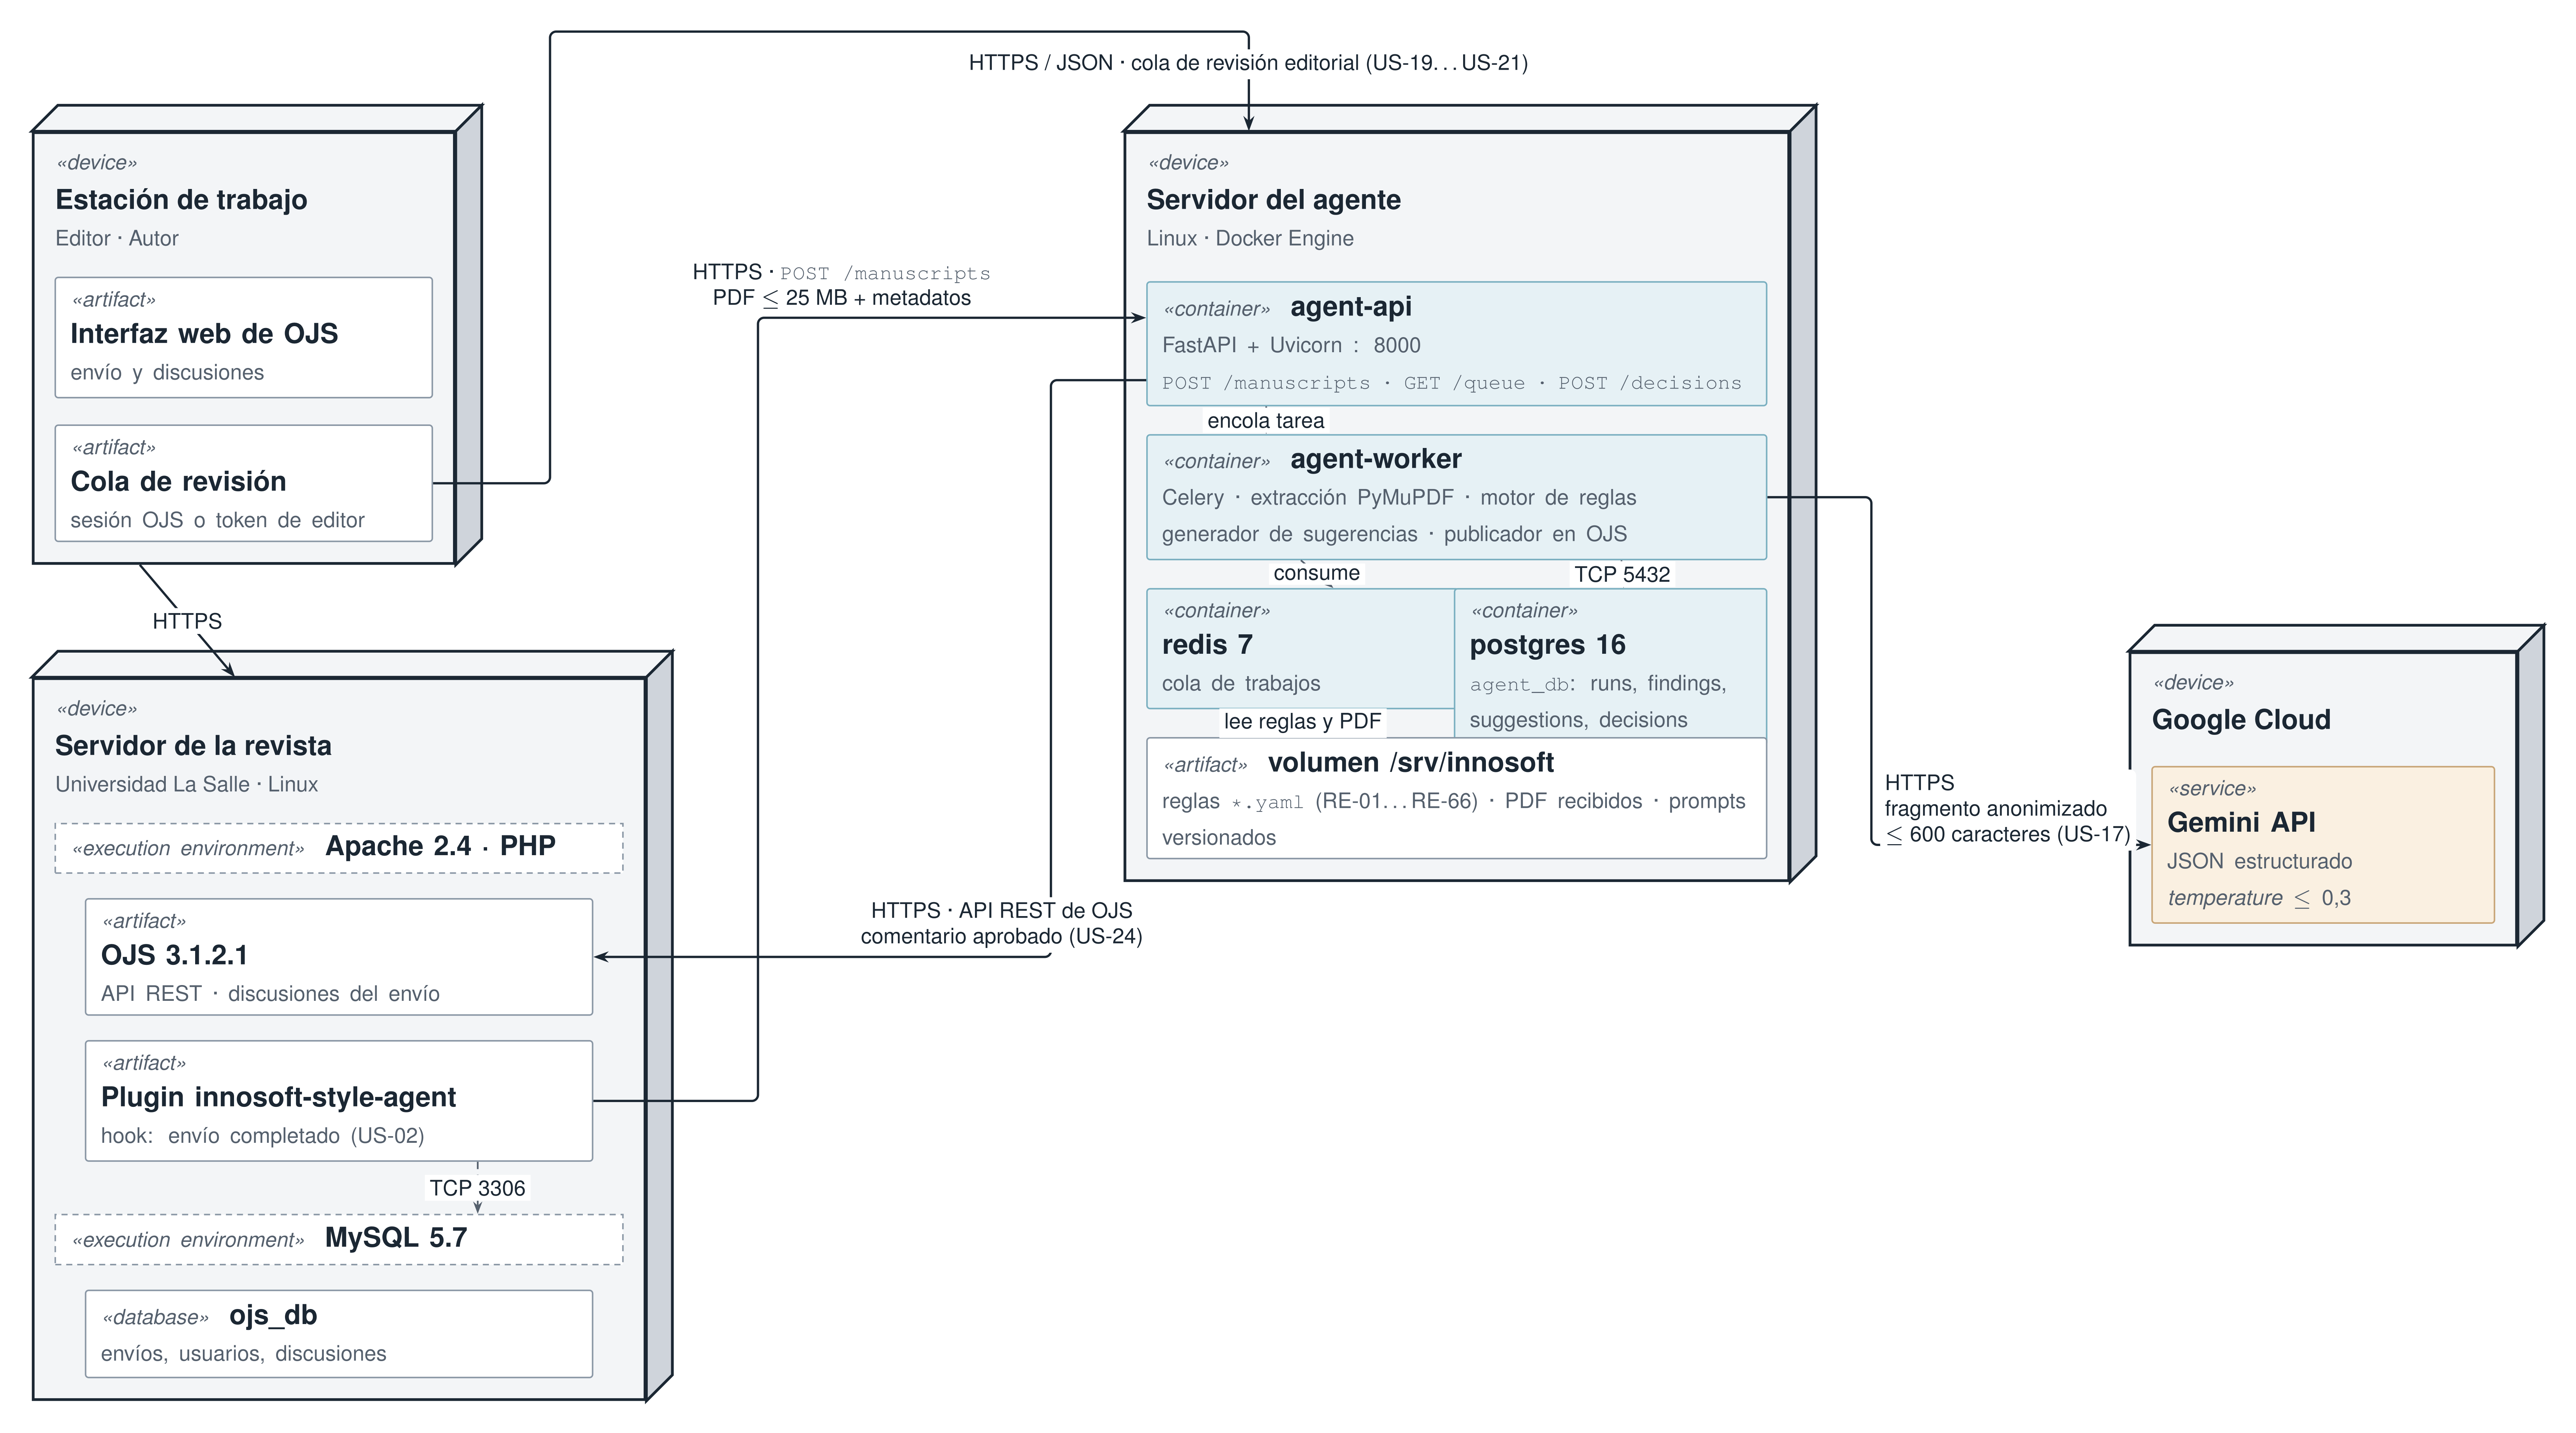
\includegraphics[width=\textwidth]{figuras/despliegue_innosoft.png}
  \caption{Diagrama de despliegue del agente integrado con OJS}
  \label{fig:despliegue}
\end{figure}

\begin{figure}[H]
  \centering
  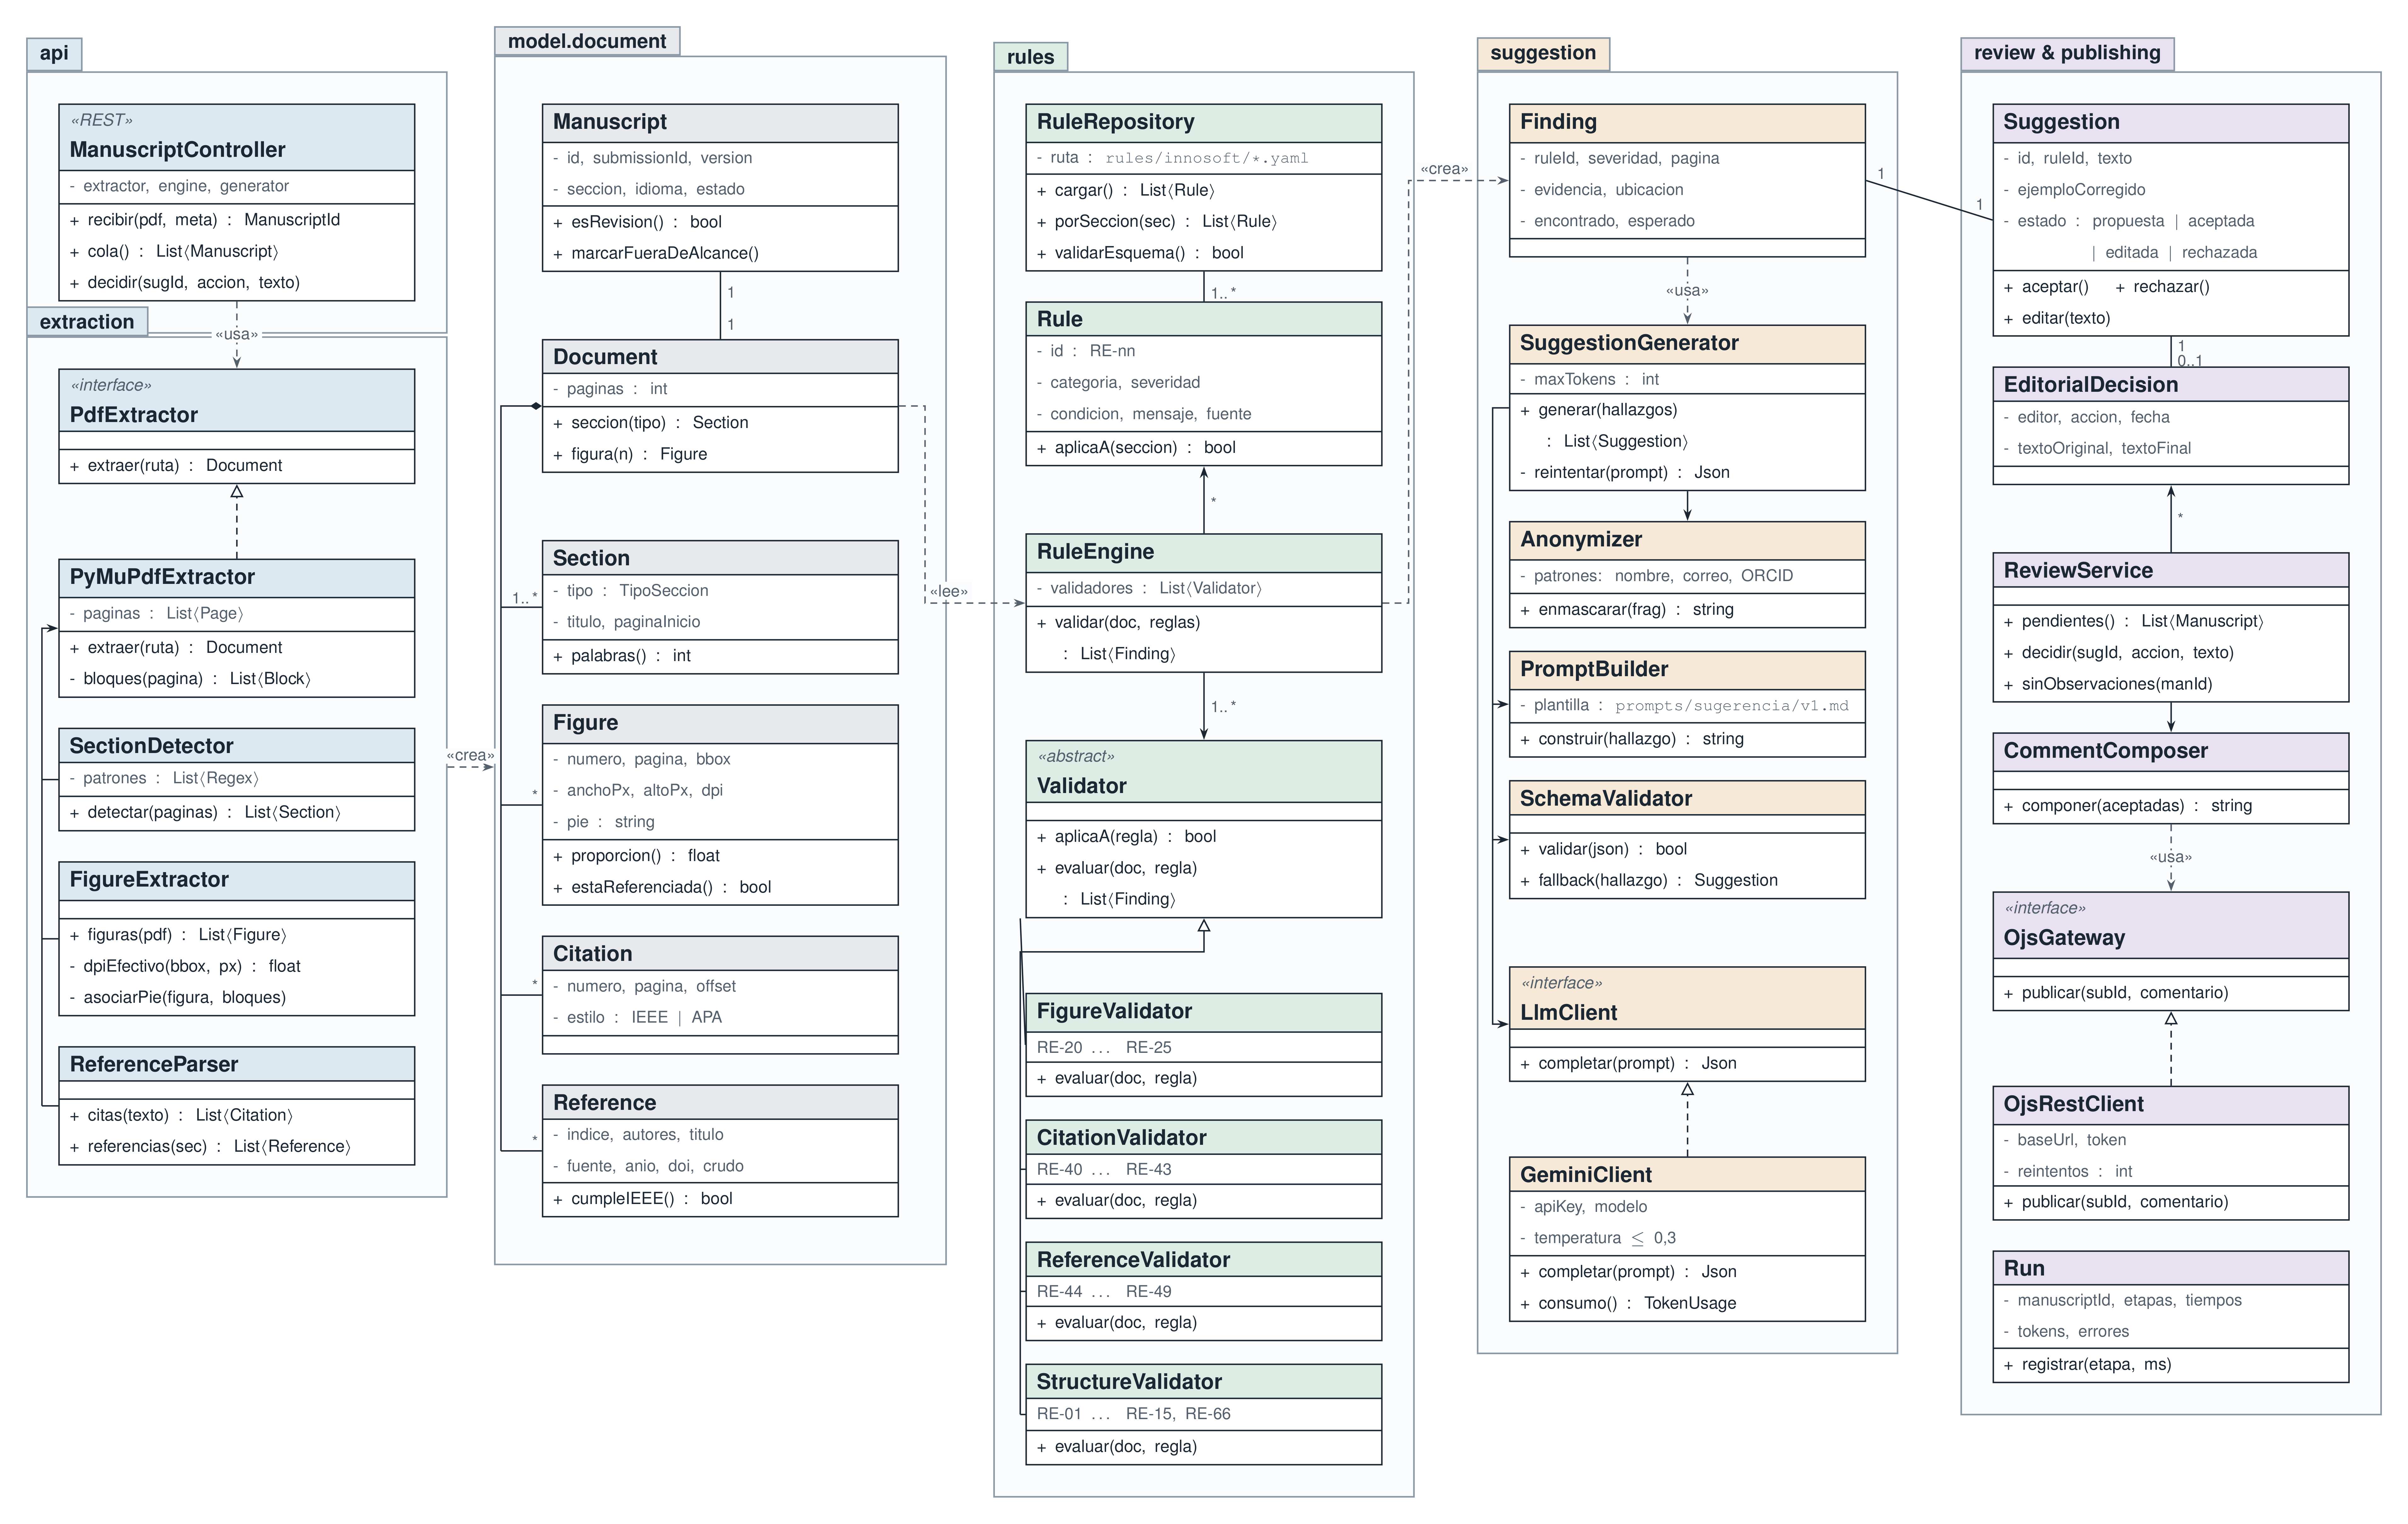
\includegraphics[width=\textwidth]{figuras/clases_innosoft.png}
  \caption{Diagrama de clases del agente}
  \label{fig:clases}
\end{figure}

\section{Plan de iteraciones}

El Sprint 1 que fue del 14 al 25 de septiembre se usó por completo en escribir las especificaciones y hacer el diseño y no produjo código. Por eso el 29 de septiembre se volvió a planificar lo que quedaba del proyecto en cinco sprints que se muestran en la Tabla~\ref{tab:3-2} y en la Figura~\ref{fig:gantt}.

{\small
\begin{longtable}{@{}>{\raggedright\arraybackslash}p{0.114\textwidth}>{\raggedright\arraybackslash}p{0.172\textwidth}>{\raggedright\arraybackslash}p{0.297\textwidth}>{\raggedright\arraybackslash}p{0.311\textwidth}@{}}
\caption{Plan por sprint (fuente: \texttt{priorizacion\_\allowbreak{}rice\_\allowbreak{}sprint1.\allowbreak{}xlsx}, hoja \emph{Replan 29-sep})}\label{tab:3-2}\\
\toprule
\textbf{Sprint} & \textbf{Fechas} & \textbf{Historias} & \textbf{Meta} \\
\midrule
\endfirsthead
\toprule
\textbf{Sprint} & \textbf{Fechas} & \textbf{Historias} & \textbf{Meta} \\
\midrule
\endhead
\bottomrule
\endfoot
\endlastfoot
1 & 14-sep $\rightarrow$ 25-sep & Catálogo, RICE, diagramas, 00-producto, formato-reglas y specs de las 37 historias & Especificación y diseño \\
2 & 29-sep $\rightarrow$ 09-oct & US-00, US-01, US-04, US-09, US-06, US-10 & \emph{Walking skeleton} en Docker con RE-20/RE-21 \\
3 & 12-oct $\rightarrow$ 23-oct & US-03, US-05\textbackslash\{\}\emph{, US-07, US-08\textbackslash\{\}}, US-11\textbackslash\{\}\emph{, US-12, US-13\textbackslash\{\}} + \emph{spike} OJS & Citas y referencias IEEE detectadas; decisión técnica sobre OJS \\
4 & 26-oct $\rightarrow$ 06-nov & US-17, US-15, US-16, US-18\textbackslash\{\}*, US-28, US-19, US-20 & Sugerencias con Gemini anonimizadas y visibles para el editor \\
5 & 09-nov $\rightarrow$ 20-nov & US-21, US-24, US-02 & El flujo completo funciona desde OJS hasta el comentario que ve el autor \\
6 & 23-nov $\rightarrow$ 04-dic & Sin historias nuevas & Evaluación (precisión, recall, F1, aceptación), manuales y tesis \\
\end{longtable}
}

Las historias marcadas con asterisco entran al producto mínimo con un alcance menor al de su especificación completa.

\begin{itemize}
  \item US-05 solo detecta Resumen Palabras clave y Referencias.
  \item US-08 separa las referencias en entradas pero no las parte en campos.
  \item US-11 solo cubre las reglas RE-23 y RE-24.
  \item US-13 solo cubre las reglas RE-44 RE-46 RE-47 y RE-49.
  \item US-18 hace reintentos pero no controla el presupuesto de tokens.
\end{itemize}

Si el proyecto vuelve a atrasarse se recorta en este orden. Primero sale el plugin de OJS de US-02 y el análisis se dispara a mano. Después US-11 pasa completa a la entrega R2. Después US-13 queda solo con RE-44 y RE-46. Y por último la evidencia que muestra US-20 queda solo en texto sin miniaturas.

\begin{figure}[H]
  \centering
  \begin{ganttchart}[
      x unit=1.2mm, y unit chart=0.65cm, y unit title=0.55cm,
      hgrid, vgrid={*{6}{draw=none}, dotted}, canvas/.style={draw=gray!50},
      time slot format=isodate,
      title/.style={fill=gray!15, draw=gray!50},
      title label font=\scriptsize,
      bar/.style={fill=gray!60, draw=gray!80},
      bar label font=\footnotesize,
      bar height=0.55,
      milestone/.style={fill=black, draw=black},
      milestone label font=\footnotesize]{2026-09-14}{2026-12-04}
    \gantttitle{Sep}{17}\gantttitle{Oct}{31}\gantttitle{Nov}{30}\gantttitle{Dic}{4} \\
    \ganttbar{S1 Especificación y diseño}{2026-09-14}{2026-09-25} \\
    \ganttbar{S2 Walking skeleton}{2026-09-29}{2026-10-09} \\
    \ganttbar{S3 Citas, referencias y spike OJS}{2026-10-12}{2026-10-23} \\
    \ganttbar{S4 Gemini e interfaz editorial}{2026-10-26}{2026-11-06} \\
    \ganttbar{S5 Revisión y publicación en OJS}{2026-11-09}{2026-11-20} \\
    \ganttbar{S6 Evaluación, manuales y tesis}{2026-11-23}{2026-12-04} \\
    \ganttmilestone{Hitos: demo (09-oct), flujo en OJS (20-nov)}{2026-10-09}
    \ganttmilestone{}{2026-11-20}
  \end{ganttchart}
  \caption{Diagrama de Gantt de los sprints según la planificación del 29 de septiembre de 2026}
  \label{fig:gantt}
\end{figure}

\section{Recursos requeridos}

{\small
\begin{longtable}{@{}>{\raggedright\arraybackslash}p{0.125\textwidth}>{\raggedright\arraybackslash}p{0.287\textwidth}>{\raggedright\arraybackslash}p{0.241\textwidth}>{\raggedright\arraybackslash}p{0.241\textwidth}@{}}
\toprule
\textbf{Tipo} & \textbf{Recursos} & \textbf{Uso} & \textbf{Disponibilidad} \\
\midrule
\endfirsthead
\toprule
\textbf{Tipo} & \textbf{Recursos} & \textbf{Uso} & \textbf{Disponibilidad} \\
\midrule
\endhead
\bottomrule
\endfoot
\endlastfoot
Humanos & Equipo de tesis, asesor, editores de Innosoft, autores participantes & Escribir y revisar reglas, programar el agente, revisar los reportes & Se coordina con la universidad y la participación es voluntaria \\
Tecnológicos & Computadoras personales, instancia de OJS, servidor del agente, PostgreSQL & Programar, integrar con OJS, hacer pruebas y guardar datos & Equipos propios y servicios gratuitos o de bajo costo \\
Software & Python, FastAPI, PyMuPDF, PostgreSQL, Pytest, Docker, Git/GitHub, API de Gemini & Procesamiento, validación, sugerencias, pruebas & Código abierto o tier gratuito \\
Información y datos & Plantillas DOCX/LaTeX, directrices, manuscritos anonimizados, corpus sintético de PDFs & Configurar reglas, probar y medir & Requiere autorización y anonimización (Ley N.º 29733) \\
Económicos & S/ 760 (Tabla~\ref{tab:2-5}) & Cuotas, despliegue, capacitación, impresiones & Financiado por el equipo \\
Metodológicos & Excel RICE, specs SDD, Sprint Backlog, encuestas de validación & Priorizar, especificar, controlar avances, evaluar & Adecuado para un equipo de dos personas \\
\end{longtable}
}

\section{Avance de la implementación}

El avance se registra por historia al cierre de cada sprint, con el estado de su especificación, sus pruebas automatizadas y su commit en el repositorio. Al cierre del Sprint 2 (9 de octubre de 2026) quedó implementado el \emph{walking skeleton} de extracción y validación: recepción de PDF por API con idempotencia (US-01), extracción de texto (US-04) y de figuras con DPI efectivo (US-06), carga de reglas YAML (US-09) y validación de figuras RE-20 y RE-21 con consulta de hallazgos (US-10), sobre el entorno Docker con integración continua (US-00): 6 de 37 historias, 2 de 44 reglas y 4 de 13 endpoints canónicos, con 84 casos de prueba en verde.

\pendiente{al cierre del Sprint 6, actualizar las cifras finales y describir lo construido en los sprints 3 a 6.}

\section{Validación y evaluación}

{\small
\begin{longtable}{@{}>{\raggedright\arraybackslash}p{0.158\textwidth}>{\raggedright\arraybackslash}p{0.231\textwidth}>{\raggedright\arraybackslash}p{0.248\textwidth}>{\raggedright\arraybackslash}p{0.257\textwidth}@{}}
\caption{Criterios de evaluación por objetivo específico}\label{tab:3-3}\\
\toprule
\textbf{Objetivo} & \textbf{Criterio} & \textbf{Método} & \textbf{Meta inicial} \\
\midrule
\endfirsthead
\toprule
\textbf{Objetivo} & \textbf{Criterio} & \textbf{Método} & \textbf{Meta inicial} \\
\midrule
\endhead
\bottomrule
\endfoot
\endlastfoot
OE1 -- Arquitectura & Módulos integrados y reglas aplicadas por revista & Prueba del flujo completo: recepción $\rightarrow$ reporte $\rightarrow$ comentario en OJS & Flujo de punta a punta en el Sprint 5 \\
OE2 -- Análisis documental & Reconocimiento de secciones, figuras, citas y referencias & Comparación con anotación manual sobre un corpus & Recall por regla $\geq$ 0,75 en reglas D \\
OE3 -- Validación y reporte & Precisión y utilidad de las sugerencias & Precisión por regla; aceptación / edición / rechazo por los editores & Precisión $\geq$ 0,85 en reglas D; aceptación $\geq$ 70 \% \\
OE4 -- Evaluación & Tiempo de análisis y de revisión estilística & Medición en \texttt{runs} (US-28) y comparación manual vs. asistida & Análisis < 3 min para 15 páginas (RNF-03); \pendiente{definir instrumento y meta de reducción del tiempo de revisión — el borrador proponía 20 \%} \\
Usabilidad del reporte & Claridad y aplicabilidad para autores y editores & Encuesta breve o juicio de expertos & Reporte valorado como útil \\
\end{longtable}
}

Las metas son propuestas del equipo y se confirman con el asesor antes del Sprint 6 (\texttt{specs/\allowbreak{}00-producto.\allowbreak{}md} §1). \pendiente{corpus anotado — número de manuscritos históricos y autorización (00-producto §18).}

\section{Aspectos éticos y protección de datos}

Los manuscritos reales pueden contener datos personales de los autores (nombres, correos, ORCID, afiliaciones). Por la Ley N.º 29733, (i) se guardan fuera del repositorio (\texttt{muestras/\allowbreak{}} en \texttt{.\allowbreak{}gitignore}), (ii) las pruebas automatizadas usan PDFs sintéticos generados con PyMuPDF, y (iii) a Gemini solo sale un fragmento de hasta 600 caracteres anonimizado, con registro de lo enviado (US-17, RNF-02).
      % Capítulo III
% % titulo: Conclusiones
% estado: pendiente
% actualizado: 2026-10-19

\begin{conclusiones}
\pendiente{redactar al cierre del Sprint 6 (23-nov a 04-dic-2026), con una conclusión por objetivo específico (OE1--OE4) sustentada en las métricas de la Tabla~\ref{tab:3-3}}

% Guía (borrar al completar):
% - OE1: ¿la arquitectura permitió agregar reglas solo con YAML? ¿cuántas reglas quedaron activas?
% - OE2: recall por tipo de elemento (secciones, figuras, citas, referencias).
% - OE3: precisión por regla y tasa de aceptación de los editores.
% - OE4: tiempo de análisis por manuscrito y comparación con la revisión manual.
% - Trabajo futuro: releases R2 y R3, otras revistas (RICCE), Celery + Redis, OCR.
\end{conclusiones}
   % Conclusiones: se incluyen al cierre del Sprint 6
% titulo: Referencias
% estado: borrador
% actualizado: 2026-10-19
% Formato IEEE. Cada entrada se cita como \cite{refN}; la numeración la asigna LaTeX en este orden.
% Para agregar una referencia: añade un \bibitem al final y cítalo en el texto.

\begin{thebibliography}{99}
\setlength{\itemsep}{4pt}
  \bibitem{ref1} S. Moutinho, “Latin American journals are open-access pioneers. Now, they need an audience,” Science, vol. 386, no. 6726, Dec. 5, 2024, doi: 10.1126/science.zjn80sl. Disponible en: \url{https://www.science.org/content/article/latin-american-journals-are-open-access-pioneers-now-they-need-audience}

  \bibitem{ref2} A. Casas Niño de Rivera, ``Opportunities for Scholarly Publishing Services in Latin America,'' M.Pub. thesis, Faculty of Communication, Art and Technology, Simon Fraser University, Burnaby, BC, Canada, Fall 2023. Disponible en: \url{https://summit.sfu.ca/_flysystem/fedora/2024-02/etd22832.pdf}

  \bibitem{ref3} M. Khalifa and M. Albadawy, “Using artificial intelligence in academic writing and research: An essential productivity tool,” Computer Methods and Programs in Biomedicine Update, vol. 5, p. 100145, Jan. 2024, doi: 10.1016/j.cmpbup.2024.100145. Disponible en: \url{https://www.sciencedirect.com/science/article/pii/S2666990024000120}

  \bibitem{ref4} P. Accuosto, F. Ronzano, D. Ferrés y H. Saggion, “Multi-level mining and visualization of scientific text collections: Exploring a bi-lingual scientific repository,” en Proceedings of the 6th International Workshop on Mining Scientific Publications (WOSP 2017), Toronto, Canada, 2017, pp. 9--16, doi: 10.1145/3127526.3127529. Disponible en: \url{https://dl.acm.org/doi/10.1145/3127526.3127529}

  \bibitem{ref5} K. A. Yaghi, “Using artificial intelligence for formatting academic journal papers,” American Academic \& Scholarly Research Journal, vol. 16, no. 4, pp. 28--57, Oct. 2024. Disponible en: \url{https://aasrc.org/aasrj/index.php/aasrj/article/view/2296}

  \bibitem{ref6} L. W. Markewich, “Extracting structured information from academic documents,” M.Sc. thesis, University of Saskatchewan, Saskatoon, SK, Canada, Apr. 11, 2022. https://harvest.usask.ca/items/d46f9406-8b3c-4999-9b39-12f472e06c4a

  \bibitem{ref7} S. Nigam, S. Verma, and P. Nagabhushan, “Document Analysis and Recognition: A Survey,” TechRxiv, Mar. 27, 2023, doi: 10.36227/techrxiv.22336435.v1. Disponible en: \url{https://www.techrxiv.org/doi/10.36227/techrxiv.22336435}

  \bibitem{ref8} DM. Minouei, M. R. Soheili, and D. Stricker, “Document layout analysis with an enhanced object detector,” in 2021 5th International Conference on Pattern Recognition and Image Analysis (IPRIA), Apr. 2021, pp. 1--5, doi: 10.1109/IPRIA53572.2021.9483509. Disponible en: \url{https://ieeexplore.ieee.org/document/9483509}

  \bibitem{ref9} S. M. B. W. Dissanayake and P. P. G. D. Asanka, “A stage-aware framework for automated IEEE research paper compliance checking using layout analysis, rule-based validation, and semantic evaluation,” in 2026 6th International Conference on Advanced Research in Computing (ICARC), Feb. 2026, pp. 1--6, doi: 10.1109/ICARC68737.2026.11454060. Disponible en: \url{https://www.researchgate.net/publication/403371900_A_Stage-Aware_Framework_for_Automated_IEEE_Research_Paper_Compliance_Checking_Using_Layout_Analysis_Rule-Based_Validation_and_Semantic_Evaluation}

  \bibitem{ref10} V. D. Tran, M. L. Nguyen, K. Shirai, and K. Satoh, “An approach of rhetorical status recognition for judgments in court documents using deep learning models,” in 2019 11th International Conference on Knowledge and Systems Engineering (KSE), Oct. 2019, pp. 1--6, doi: 10.1109/KSE.2019.8919370. Disponible en: \url{https://ieeexplore.ieee.org/document/8919370}

  \bibitem{ref11} S. Dündar, “Performance analysis of text chunking methods for LLM-based document summarization,” IEEE Xplore, Sep. 2025. Disponible en: \url{https://ieeexplore.ieee.org/document/11206896}

  \bibitem{ref12} J. Ye and K. Xu, “UDMtext: A unified deep mutual learning-based framework for text detection in complex documents,” in 2025 6th International Conference on Computer Vision, Image and Deep Learning (CVIDL), May 2025, doi: 10.1109/CVIDL65390.2025.11086049. Disponible en: \url{https://www.researchgate.net/publication/394005168_UDMtext_a_Unified_Deep_Mutual_Learning-Based_Framework_for_Text_Detection_in_Complex_Documents}

  \bibitem{ref13} M. Moskalev and T. T. Gazizov, “AI-based algorithm for significant information extraction from unstructured textual data,” in 2025 International Russian Automation Conference (RusAutoCon), Sep. 2025, doi: 10.1109/RusAutoCon65989.2025.11177408. Disponible en: \url{https://www.researchgate.net/publication/396022201_AI-Based_Algorithm_for_Significant_Information_Extraction_from_Unstructured_Textual_Data}

  \bibitem{ref14} R. Poorvadevi, H. Surendar, and S. SriRamakrishnan, “Effective analysis of data processing on cloud using serverless computing,” in 2025 8th International Conference on Trends in Electronics and Informatics (ICOEI), Apr. 2025, doi: 10.1109/ICOEI65986.2025.11013090. Disponible en: \url{https://www.researchgate.net/publication/392245936_Effective_Analysis_of_Data_Processing_on_Cloud_using_Serverless_Computing}

  \bibitem{ref15} J. Chen, S. Yang, and S. Jiang, “Automatic classification and recognition of complex documents based on Faster RCNN,” in 2019 14th IEEE International Conference on Electronic Measurement \& Instruments (ICEMI), Nov. 2019, pp. 573--577, doi: 10.1109/ICEMI46757.2019.9101847. Disponible en: \url{https://www.researchgate.net/publication/341695915_Automatic_classification_and_recognition_of_complex_documents_based_on_Faster_RCNN}

  \bibitem{ref16} S. Takeshita, T. Green, N. Friedrich, K. Eckert, and S. P. Ponzetto, “X-SCITLDR: Cross-lingual extreme summarization of scholarly documents,” in Proceedings of the ACM/IEEE Joint Conference on Digital Libraries (JCDL 2022), Cologne, Germany, Jun. 20--24, 2022, doi: 10.1145/3529372.3530938.

  \bibitem{ref17} W. Ma, M. Cao, J. Ma, Z. Dong, C. Yang, and Z. Li, “Mamba-YOLO: Multi-level adaptive rectangular convolution for document layout analysis,” Pattern Recognition, vol. 170, Art. no. 112031, Feb. 2026, doi: 10.1016/j.patcog.2025.112031.

  \bibitem{ref18} L. Pisaneschi, A. Gemelli, and S. Marinai, “Automatic generation of scientific papers for data augmentation in document layout analysis,” Pattern Recognition Letters, vol. 167, pp. 38--44, 2023, doi: 10.1016/j.patrec.2023.01.018.

  \bibitem{ref19} X. Wu et al., “Cross-domain document layout analysis using document style guide,” Expert Systems with Applications, vol. 245, Art. no. 123039, Jul. 2024, doi: 10.1016/j.eswa.2023.123039.

  \bibitem{ref20} A. Peña et al., “Continuous document layout analysis: Human-in-the-loop AI-based data curation, database, and evaluation in the domain of public affairs,” Information Fusion, vol. 108, Art. no. 102398, Aug. 2024, doi: 10.1016/j.inffus.2024.102398.

  \bibitem{ref21} P. Mishra, “Domain adaptive learning for document layout analysis and object detection using classifier alignment mechanism,” Signal Processing: Image Communication, vol. 116, Art. no. 116986, Aug. 2023, doi: 10.1016/j.image.2023.116986.

  \bibitem{ref22} N. Raman, S. Shah, and M. Veloso, “Synthetic document generator for annotation-free layout recognition,” Pattern Recognition, vol. 128, Art. no. 108660, Aug. 2022, doi: 10.1016/j.patcog.2022.108660.

  \bibitem{ref23} K. Nandi and S. S. Sathya, “Visual document understanding: A comparative review of modern methods,” in Computer Vision and Image Processing, Communications in Computer and Information Science, pp. 411--427, 2026, doi: 10.1007/978-3-031-93694-4\_29.

  \bibitem{ref24} C. Xu, Y. Li, S. Cao, H. Zhang, H. Bi, and Y. Chen, “HiM: Hierarchical multimodal network for document layout analysis,” Applied Intelligence, vol. 53, no. 20, pp. 24314--24326, Jul. 2023, doi: 10.1007/s10489-023-04782-3.

  \bibitem{ref25} R.-Y. Cao, Y.-X. Cao, G.-B. Zhou, and P. Luo, “Extracting variable-depth logical document hierarchy from long documents,” Journal of Computer Science and Technology, vol. 37, no. 3, pp. 699--718, May 2022, doi: 10.1007/s11390-021-1076-7.

  \bibitem{ref26} P. Constantopoulos and V. Pertsas, “From publications to knowledge graphs,” in Communications in Computer and Information Science, 2020, pp. 18--33, doi: 10.1007/978-3-030-44900-1\_2.

  \bibitem{ref27} Z. Chkirbene, R. Hamila, A. Gouissem, and U. Devrim, “Large language models (LLM) in industry: A survey of applications, challenges, and trends,” in 2024 19th International Conference on High Performance Computing \& Simulation / HONET, Dec. 2024, pp. 229--234, doi: 10.1109/HONET63146.2024.10822885.

  \bibitem{ref28} L. Wang et al., “A survey on large language model based autonomous agents,” arXiv preprint arXiv:2308.11432, Aug. 2023.

  \bibitem{ref29} D. J. Anderson, Kanban: Successful Evolutionary Change for Your Technology Business. Sequim, WA, USA: Blue Hole Press, Apr. 2010.

\end{thebibliography}

% Pendientes de cita (añadir como \bibitem y citar):
% - Guía de Scrum (Schwaber y Sutherland) — 2.1.3 y 3.2
% - Método RICE (Intercom) — 2.1.3 y 3.2
% - Spec-Driven Development — 2.1.3 y 3.2
% - Documentación de OJS 3.x / PKP (API REST y plugins)
% - Ley N.º 29733, Ley de Protección de Datos Personales (Perú) — 3.11
% Observaciones: ref3 (Khalifa y Albadawy) no se cita en el cuerpo; ref29 (Kanban) quedó sin uso al adoptar Scrum.         % Referencias (thebibliography, IEEE)

\anexos
% titulo: Anexo A – Ficha de búsqueda
% estado: borrador
% actualizado: 2026-10-19
% Procede de la sección "Revisión y fundamentación teórica" del borrador original (Tesis2026.pdf).

\anexo{Ficha de búsqueda}\label{anexo:A}

La búsqueda de antecedentes se realizó entre septiembre y octubre de 2026 en bases de datos de editoriales (ACM, IEEE, ScienceDirect, SpringerLink), motores de indexación (Google Scholar, Web of Science, Scopus) y el repositorio nacional de tesis ALICIA. La Tabla~\ref{tab:busqueda} registra la cadena usada en cada fuente y el número de documentos que superó cada filtro: T = resultados totales, 1f = filtro por título, 2f = filtro por resumen, 3f = filtro por contenido.

{\scriptsize
\begin{longtable}{@{}>{\raggedright\arraybackslash}p{0.073\textwidth}>{\raggedright\arraybackslash}p{0.117\textwidth}>{\raggedright\arraybackslash}p{0.073\textwidth}>{\raggedright\arraybackslash}p{0.073\textwidth}>{\raggedright\arraybackslash}p{0.073\textwidth}>{\raggedright\arraybackslash}p{0.073\textwidth}>{\raggedright\arraybackslash}p{0.333\textwidth}@{}}
\caption{Ficha de búsqueda: bases de datos, cadenas y resultados por filtro}\label{tab:busqueda}\\
\toprule
\textbf{Cód.} & \textbf{Base de datos} & \textbf{T} & \textbf{1f} & \textbf{2f} & \textbf{3f} & \textbf{Cadena de búsqueda} \\
\midrule
\endfirsthead
\toprule
\textbf{Cód.} & \textbf{Base de datos} & \textbf{T} & \textbf{1f} & \textbf{2f} & \textbf{3f} & \textbf{Cadena de búsqueda} \\
\midrule
\endhead
\bottomrule
\endfoot
\endlastfoot
ACM & ACM Digital Library & 9 & 1 & 1 & 1 & (``artificial intelligence'' OR AI OR ``machine learning'' OR NLP) AND (format OR formatting OR ``style compliance'' OR ``layout error'') AND (detection OR automatic OR validation OR checking) AND (``academic article'' OR ``journal article'' OR ``research paper'') AND (``Open Journal Systems'' OR OJS) \\
IEEE & IEEE Xplore Digital Library & 89 & 86 & 29 & 9 & (``document layout analysis'' OR ``document structure analysis'' OR ``document processing'') AND (``natural language processing'' OR NLP OR ``deep learning'') AND (automatic OR automated) \\
SD & ScienceDirect & 9 & 9 & 6 & 6 & (``document layout analysis'' OR ``document structure extraction'') AND (``scientific articles'' OR ``academic papers'') AND (``deep learning'' OR ``NLP'') AND (``information extraction'' OR ``document understanding'') \\
SPL & SpringerLink & 11 & 5 & 5 & 4 & (``document structure extraction'' OR ``document layout analysis'' OR ``text structure'') AND (``scientific articles'' OR ``research papers'') AND (``NLP'' OR ``deep learning'') AND (``information extraction'' OR ``document understanding'') \\
GS & Google Scholar & 14 & 8 & 6 & 4 & (``automatic formatting'' OR ``document structure analysis'') AND (``scientific articles'' OR ``academic journals'') AND (``natural language processing'' OR ``machine learning'') AND (OJS OR ``Open Journal Systems'' OR Spanish OR ``Latin America'') \\
WS & Web of Science & --- & --- & --- & --- & \pendiente{ejecutar la búsqueda o retirar la fila} \\
SC & Scopus & --- & --- & --- & --- & \pendiente{ejecutar la búsqueda o retirar la fila} \\
ALICIA & Repositorio ALICIA (tesis) & 0 & 0 & 0 & 0 & (``scientific article format'' OR ``academic writing'') AND (``scientific journals'' OR ``thesis'') \\
 & \textbf{Total} & \textbf{132} & \textbf{109} & \textbf{47} & \textbf{24} &  \\
\end{longtable}
}

\subsubsection*{Criterios de selección}

Para filtrar los 132 resultados se aplicaron cuatro criterios de forma secuencial, tanto a artículos como a tesis:

\begin{itemize}
  \item \textbf{Prefiltrado (T = 132):} se descartan los documentos que no son artículos científicos ni tesis (editoriales, reseñas, llamados a publicación).
  \item \textbf{Filtro por título (1f = 109):} se conservan los documentos cuyo título tiene relación directa con la investigación.
  \item \textbf{Filtro por resumen (2f = 47):} se seleccionan los documentos cuyo resumen confirma que el trabajo es relevante.
  \item \textbf{Filtro por contenido (3f = 24):} se revisa el cuerpo del documento y se conservan los que aportan métodos, evidencia o referentes aplicables al agente propuesto. De los 24, GS-13 es un registro institucional duplicado de GS-10, por lo que se analizan \textbf{23 estudios independientes}.
\end{itemize}

% Disponibles pero fuera del documento (decisión del 19-oct-2026):
% % titulo: Anexo A – Fichas de lectura crítica
% estado: no incluido
% actualizado: 2026-10-19

\anexo{Fichas de lectura crítica}

Cada ficha registra, para un documento seleccionado en el filtro por contenido (3f), el problema, la solución, los resultados, las limitaciones y las conclusiones, con su aporte a la tesis. GS-13 es un duplicado institucional de GS-10 y no se cuenta como estudio independiente.

\subsubsection*{ACM-03. Multi-level mining and visualization of scientific text collections}

\begin{longtable}{@{}>{\raggedright\arraybackslash}p{0.173\textwidth}>{\raggedright\arraybackslash}p{0.774\textwidth}@{}}
\toprule
\textbf{Campo} & \textbf{Descripción} \\
\midrule
\endfirsthead
\toprule
\textbf{Campo} & \textbf{Descripción} \\
\midrule
\endhead
\bottomrule
\endfoot
\endlastfoot
Problema & El volumen de publicaciones científicas crece demasiado rápido para que los investigadores se mantengan al día. Las herramientas existentes pierden información estructural al procesar PDFs y los servicios bibliográficos tienen baja cobertura sobre afiliaciones de autores. \\
Solución & Sistema web que extrae contenido de PDFs preservando su estructura, identifica autores y afiliaciones geográficas, clasifica oraciones por función retórica, modela tópicos con LDA y ofrece visualizaciones interactivas (mapas, grafos, histogramas). Aplicado al corpus bilingüe SEPLN (505 artículos, 2008--2016). \\
Resultados & Extractor de PDF con F1 = 0.917. Identificación de afiliaciones con precisión de 0.83 (URI) y 0.91 (país). Plataforma web funcional con búsqueda facetada y 7 visualizaciones. El caso de estudio detectó un cambio terminológico de ``sentiment analysis'' a ``opinion mining'' en 2014. \\
Limitaciones & El extractor falla con formatos atípicos. Los tópicos LDA solo se generaron en inglés (posible sesgo). El clasificador retórico no funciona en español. No se hizo validación con usuarios ni pruebas de escalabilidad. \\
Conclusiones & Las herramientas de análisis profundo más visualizaciones flexibles permiten explotar mejor el conocimiento de colecciones científicas. El sistema enriquece artículos con metadatos, semántica e información retórica, y se publicará como librería abierta. Aporte clave: enfoque multilingüe (inglés-español). \\
\end{longtable}

\subsubsection*{GS-01. Using artificial intelligence for formatting academic journal papers}

\begin{longtable}{@{}>{\raggedright\arraybackslash}p{0.202\textwidth}>{\raggedright\arraybackslash}p{0.745\textwidth}@{}}
\toprule
\textbf{Campo} & \textbf{Descripción} \\
\midrule
\endfirsthead
\toprule
\textbf{Campo} & \textbf{Descripción} \\
\midrule
\endhead
\bottomrule
\endfoot
\endlastfoot
Problema & Los investigadores enfrentan dificultades y pérdida de tiempo en el formateo manual de artículos para revistas académicas. \\
Solución & Sistema de formateo automático basado en IA para papers académicos orientado a mejorar productividad, consistencia y credibilidad. Herramientas: IA, formateo automático, journals académicos, machine learning. \\
Resultados & Sistema de formateo automático viable para papers académicos con mejoras en productividad y consistencia. \\
Limitaciones & No especifica implementación en OJS ni foco en español o journals latinoamericanos. \\
Conclusiones & El estudio responde al problema mediante una propuesta aplicable al análisis documental. Su aporte para la tesis (RQ1, RQ2, RQ3) es ser el antecedente más directo de la propuesta de tesis; referente fundamental para justificar la necesidad del agente. \\
\end{longtable}

\subsubsection*{GS-10. Extracting Structured Information From Academic Documents}

\begin{longtable}{@{}>{\raggedright\arraybackslash}p{0.206\textwidth}>{\raggedright\arraybackslash}p{0.741\textwidth}@{}}
\toprule
\textbf{Campo} & \textbf{Descripción} \\
\midrule
\endfirsthead
\toprule
\textbf{Campo} & \textbf{Descripción} \\
\midrule
\endhead
\bottomrule
\endfoot
\endlastfoot
Problema & Los documentos académicos contienen información estructurada no trivial de extraer automáticamente. \\
Solución & Métodos de extracción de información estructurada y relaciones aplicados a documentos académicos; uso del dataset DAD. Herramientas: NLP, extracción de información, análisis de estructura, documentos académicos. \\
Resultados & Extracción efectiva de información estructurada de artículos académicos mediante NLP y análisis de estructura. \\
Limitaciones & No aborda formateo automático ni integración con OJS ni español. \\
Conclusiones & El estudio responde al problema mediante una propuesta aplicable al análisis documental. Su aporte para la tesis (RQ1) es una metodología de extracción de información estructurada de papers académicos directamente aplicable al agente. \\
\end{longtable}

\subsubsection*{GS-11. Document analysis and recognition: a survey}

\begin{longtable}{@{}>{\raggedright\arraybackslash}p{0.211\textwidth}>{\raggedright\arraybackslash}p{0.736\textwidth}@{}}
\toprule
\textbf{Campo} & \textbf{Descripción} \\
\midrule
\endfirsthead
\toprule
\textbf{Campo} & \textbf{Descripción} \\
\midrule
\endhead
\bottomrule
\endfoot
\endlastfoot
Problema & La multiplicidad de métodos en análisis y reconocimiento de documentos requiere una revisión sistemática. \\
Solución & Encuesta de métodos de análisis y reconocimiento de documentos incluyendo OCR, ML y deep learning. Herramientas: OCR, machine learning, deep learning, análisis de documentos, reconocimiento. \\
Resultados & El OCR combinado con ML y deep learning mejora el análisis de estructura de documentos. \\
Limitaciones & Preprint; no específico a artículos científicos en español. \\
Conclusiones & El estudio responde al problema mediante una propuesta aplicable al análisis documental. Su aporte para la tesis (RQ1) es una base técnica amplia sobre análisis de documentos para fundamentar las tecnologías del agente. \\
\end{longtable}

\subsubsection*{GS-13. Extracting Structured Information From Academic Documents (institutional record)}

\begin{longtable}{@{}>{\raggedright\arraybackslash}p{0.257\textwidth}>{\raggedright\arraybackslash}p{0.690\textwidth}@{}}
\toprule
\textbf{Campo} & \textbf{Descripción} \\
\midrule
\endfirsthead
\toprule
\textbf{Campo} & \textbf{Descripción} \\
\midrule
\endhead
\bottomrule
\endfoot
\endlastfoot
Problema & Duplicado institucional de GS-10. \\
Solución & Ver GS-10. Herramientas: NLP, extracción de información estructurada, documentos académicos. \\
Resultados & Ver GS-10. \\
Limitaciones & Es duplicado institucional de GS-10; no debe contarse como estudio independiente. \\
Conclusiones & La fuente confirma la disponibilidad institucional de GS-10, pero no aporta un estudio nuevo. Para evitar duplicidad, debe citarse solo como respaldo o acceso alternativo. \\
\end{longtable}

\subsubsection*{IEEE-01. Document Layout Analysis with an Enhanced Object Detector}

\begin{longtable}{@{}>{\raggedright\arraybackslash}p{0.208\textwidth}>{\raggedright\arraybackslash}p{0.739\textwidth}@{}}
\toprule
\textbf{Campo} & \textbf{Descripción} \\
\midrule
\endfirsthead
\toprule
\textbf{Campo} & \textbf{Descripción} \\
\midrule
\endhead
\bottomrule
\endfoot
\endlastfoot
Problema & Extracción automática de contenido en imágenes de documentos; delimitación de regiones como párrafos, figuras y tablas. \\
Solución & Red neuronal convolucional (inspirada en detectores de escenas naturales) entrenada en dataset público para análisis de layout. Herramientas: CNN, deep learning, OCR, detección de objetos. \\
Resultados & El método demuestra el potencial de detectores de objetos para análisis de layout de documentos. \\
Limitaciones & Evaluado solo en dataset público; no aborda documentos científicos multilingües ni en español. \\
Conclusiones & El estudio responde al problema mediante una propuesta aplicable al análisis documental. Su aporte para la tesis (RQ1) es una base técnica para análisis de layout de artículos científicos. \\
\end{longtable}

\subsubsection*{IEEE-13. A Stage-Aware Framework for Automated IEEE Research Paper Compliance Checking Using Layout Analysis, Rule-Based Validation, and Semantic Evaluation}

\begin{longtable}{@{}>{\raggedright\arraybackslash}p{0.196\textwidth}>{\raggedright\arraybackslash}p{0.751\textwidth}@{}}
\toprule
\textbf{Campo} & \textbf{Descripción} \\
\midrule
\endfirsthead
\toprule
\textbf{Campo} & \textbf{Descripción} \\
\midrule
\endhead
\bottomrule
\endfoot
\endlastfoot
Problema & Las verificaciones manuales de cumplimiento de formato IEEE son lentas, subjetivas y propensas a omisiones. \\
Solución & Framework híbrido con análisis de layout (PubLayNet), motor de reglas YAML y evaluación semántica (SciBERT) para validar cumplimiento de formato IEEE. Herramientas: PubLayNet, SciBERT, YAML, análisis de layout, validación de reglas. \\
Resultados & Rendimiento fuerte en detección de secciones, validación de layout y verificación de reglas; >85\% de acuerdo con evaluación humana en 15 papers. \\
Limitaciones & Evaluado solo en papers IEEE; no adaptado a otros estilos ni a journals latinoamericanos o en español. \\
Conclusiones & El estudio responde al problema mediante una propuesta aplicable al análisis documental. Su aporte para la tesis (RQ1, RQ2, RQ3) es ser el caso más cercano al sistema propuesto; referente directo para validación automática de formato en artículos científicos. \\
\end{longtable}

\subsubsection*{SPL-09. From Publications to Knowledge Graphs}

\begin{longtable}{@{}>{\raggedright\arraybackslash}p{0.202\textwidth}>{\raggedright\arraybackslash}p{0.745\textwidth}@{}}
\toprule
\textbf{Campo} & \textbf{Descripción} \\
\midrule
\endfirsthead
\toprule
\textbf{Campo} & \textbf{Descripción} \\
\midrule
\endhead
\bottomrule
\endfoot
\endlastfoot
Problema & La información en publicaciones científicas no está conectada de forma semántica ni es explotable automáticamente. \\
Solución & Pipeline para transformar publicaciones científicas en grafos de conocimiento mediante extracción de entidades y relaciones. Herramientas: Grafos de conocimiento, extracción de información, NLP, publicaciones científicas. \\
Resultados & Propone convertir publicaciones científicas en grafos de conocimiento mediante extracción de entidades, relaciones y metadatos. \\
Limitaciones & Abstract no disponible; no orientado a formateo ni a OJS. \\
Conclusiones & El estudio responde al problema mediante una propuesta aplicable al análisis documental. Su aporte para la tesis (RQ1) es ser relevante para enriquecer metadatos de artículos en el contexto del agente (entidades, relaciones, citas). \\
\end{longtable}

\subsubsection*{IEEE-16. An Approach of Rhetorical Status Recognition for Judgments in Court Documents using Deep Learning Models}

\begin{longtable}{@{}>{\raggedright\arraybackslash}p{0.210\textwidth}>{\raggedright\arraybackslash}p{0.737\textwidth}@{}}
\toprule
\textbf{Campo} & \textbf{Descripción} \\
\midrule
\endfirsthead
\toprule
\textbf{Campo} & \textbf{Descripción} \\
\midrule
\endhead
\bottomrule
\endfoot
\endlastfoot
Problema & Falta de análisis automático de estructura retórica en documentos legales para apoyar sistemas de recuperación. \\
Solución & Modelos de deep learning para clasificar el estado retórico de cada oración en documentos judiciales. Herramientas: Deep learning, LSTM, redes neuronales, NLP. \\
Resultados & Resultados prometedores sugieren la aplicabilidad de módulos de redes neuronales con información retórica. \\
Limitaciones & Dominio legal específico; no generalizable directamente a artículos científicos. \\
Conclusiones & El estudio responde al problema mediante una propuesta aplicable al análisis documental. Su aporte para la tesis (RQ1) es una analogía útil para clasificación de secciones retóricas en artículos científicos. \\
\end{longtable}

\subsubsection*{IEEE-37. Performance Analysis of Text Chunking Methods for LLM-Based Document Summarization}

\begin{longtable}{@{}>{\raggedright\arraybackslash}p{0.210\textwidth}>{\raggedright\arraybackslash}p{0.737\textwidth}@{}}
\toprule
\textbf{Campo} & \textbf{Descripción} \\
\midrule
\endfirsthead
\toprule
\textbf{Campo} & \textbf{Descripción} \\
\midrule
\endhead
\bottomrule
\endfoot
\endlastfoot
Problema & Ventana de contexto limitada de los LLMs para documentos extensos. \\
Solución & Comparación de cuatro estrategias de chunking (Fixed-Length, Recursive, Sliding Window, Semantic) sobre dos LLMs y dos datasets. Herramientas: LLMs, Llama 3.1, Phi-4, chunking, ROUGE, BLEU. \\
Resultados & Sliding Window y Semantic Chunking superan a Recursive; resultados dependen del modelo y del dataset. \\
Limitaciones & Evaluado en dominios gubernamentales y legales; no en artículos científicos en español. \\
Conclusiones & El estudio responde al problema mediante una propuesta aplicable al análisis documental. Su aporte para la tesis (RQ1, RQ3) son estrategias aplicables al procesamiento de manuscritos científicos extensos en el agente propuesto. \\
\end{longtable}

\subsubsection*{IEEE-38. UDMtext: a Unified Deep Mutual Learning-Based Framework for Text Detection in Complex Documents}

\begin{longtable}{@{}>{\raggedright\arraybackslash}p{0.211\textwidth}>{\raggedright\arraybackslash}p{0.736\textwidth}@{}}
\toprule
\textbf{Campo} & \textbf{Descripción} \\
\midrule
\endfirsthead
\toprule
\textbf{Campo} & \textbf{Descripción} \\
\midrule
\endhead
\bottomrule
\endfoot
\endlastfoot
Problema & Los métodos OCR existentes tienen baja robustez ante documentos con layouts complejos. \\
Solución & Framework UDMtext con modelo maestro y dos modelos estudiante con aprendizaje mutuo y función de pérdida híbrida. Herramientas: Deep learning, OCR, mutual learning, knowledge distillation, ICDAR. \\
Resultados & 72.91\% de accuracy y 62.31\% de recall en ICDAR 2023; mayor robustez en layouts complejos. \\
Limitaciones & Evaluado en ICDAR 2023; no específico a artículos científicos ni a español. \\
Conclusiones & El estudio responde al problema mediante una propuesta aplicable al análisis documental. Su aporte para la tesis (RQ1) es una técnica aplicable para mejorar extracción de texto en manuscritos con layouts complejos. \\
\end{longtable}

\subsubsection*{IEEE-51. AI-Based Algorithm for Significant Information Extraction from Unstructured Textual Data}

\begin{longtable}{@{}>{\raggedright\arraybackslash}p{0.207\textwidth}>{\raggedright\arraybackslash}p{0.740\textwidth}@{}}
\toprule
\textbf{Campo} & \textbf{Descripción} \\
\midrule
\endfirsthead
\toprule
\textbf{Campo} & \textbf{Descripción} \\
\midrule
\endhead
\bottomrule
\endfoot
\endlastfoot
Problema & Volumen creciente de información no estructurada que requiere métodos eficientes de extracción. \\
Solución & Algoritmo con redes neuronales artificiales y bibliotecas de visión computacional que devuelve resultados en JSON sin depender de plantillas fijas. Herramientas: Redes neuronales, visión computacional, JSON, NLP. \\
Resultados & Reducción significativa del tiempo de procesamiento manual de documentos de texto. \\
Limitaciones & No evaluado en artículos científicos en español ni integrado con flujos editoriales. \\
Conclusiones & El estudio responde al problema mediante una propuesta aplicable al análisis documental. Su aporte para la tesis (RQ1, RQ3) es un enfoque de extracción sin plantillas relevante para la adaptabilidad del agente a distintos estilos de revista. \\
\end{longtable}

\subsubsection*{IEEE-54. Effective Analysis of Data Processing on Cloud using Serverless Computing}

\begin{longtable}{@{}>{\raggedright\arraybackslash}p{0.203\textwidth}>{\raggedright\arraybackslash}p{0.744\textwidth}@{}}
\toprule
\textbf{Campo} & \textbf{Descripción} \\
\midrule
\endfirsthead
\toprule
\textbf{Campo} & \textbf{Descripción} \\
\midrule
\endhead
\bottomrule
\endfoot
\endlastfoot
Problema & Necesidad de gestionar y analizar eficientemente documentos (PDFs, CSVs, Excel) en ecosistemas digitales. \\
Solución & Arquitectura serverless con AWS Lambda y Gemini AI para extracción y análisis de contenido multiformat con respuestas en tiempo real. Herramientas: AWS Lambda, Google Gemini AI, serverless, NLP, procesamiento de documentos. \\
Resultados & Flujos de gestión documental optimizados con mayor accesibilidad y comprensión de texto no estructurado. \\
Limitaciones & No orientado a artículos científicos ni a estándares editoriales latinoamericanos. \\
Conclusiones & El estudio responde al problema mediante una propuesta aplicable al análisis documental. Su aporte para la tesis (RQ1, RQ3) es una arquitectura de referencia para el despliegue del agente de formateo en entornos cloud. \\
\end{longtable}

\subsubsection*{IEEE-55. Automatic classification and recognition of complex documents based on Faster RCNN}

\begin{longtable}{@{}>{\raggedright\arraybackslash}p{0.204\textwidth}>{\raggedright\arraybackslash}p{0.743\textwidth}@{}}
\toprule
\textbf{Campo} & \textbf{Descripción} \\
\midrule
\endfirsthead
\toprule
\textbf{Campo} & \textbf{Descripción} \\
\midrule
\endhead
\bottomrule
\endfoot
\endlastfoot
Problema & Los sistemas OCR convencionales fallan con documentos complejos que contienen información no textual. \\
Solución & Pipeline con Faster RCNN (RPN + clasificación de regiones) para segmentar y reconocer automáticamente regiones en documentos complejos. Herramientas: Faster RCNN, RPN, OCR, deep learning, segmentación de documentos. \\
Resultados & Separación precisa de áreas de sello, texto y número de página; mejora del pipeline OCR posterior. \\
Limitaciones & Evaluado en documentos simples; no probado en artículos científicos multicolumna en español. \\
Conclusiones & El estudio responde al problema mediante una propuesta aplicable al análisis documental. Su aporte para la tesis (RQ1) es una técnica de segmentación regional aplicable al preprocesamiento de manuscripts científicos. \\
\end{longtable}

\subsubsection*{IEEE-62. X-SCITLDR: Cross-Lingual Extreme Summarization of Scholarly Documents}

\begin{longtable}{@{}>{\raggedright\arraybackslash}p{0.196\textwidth}>{\raggedright\arraybackslash}p{0.751\textwidth}@{}}
\toprule
\textbf{Campo} & \textbf{Descripción} \\
\midrule
\endfirsthead
\toprule
\textbf{Campo} & \textbf{Descripción} \\
\midrule
\endhead
\bottomrule
\endfoot
\endlastfoot
Problema & La investigación previa en summarización de papers se ha concentrado solo en inglés; no existe soporte multilingüe. \\
Solución & Dataset XSCITLDR para summarización multilingüe y modelos basados en mBART; incluye enfoque 'summarize and translate' y modelo cross-lingual directo. Herramientas: mBART, summarización cross-lingüística, NLP multilingüe, SCITLDR. \\
Resultados & Presenta X-SCITLDR para resumir documentos académicos de forma cross-lingüística. Los modelos directos fueron competitivos frente al proceso de resumir y traducir. \\
Limitaciones & No incluye español ni portugués; se centra en alemán, italiano, chino y japonés. \\
Conclusiones & El estudio responde al problema mediante una propuesta aplicable al análisis documental. Su aporte para la tesis (RQ2, RQ3) es ser un referente metodológico clave para adaptar modelos de procesamiento de papers científicos al español. \\
\end{longtable}

\subsubsection*{SD-04. Mamba-YOLO: Multi-level adaptive rectangular convolution for Document Layout Analysis}

\begin{longtable}{@{}>{\raggedright\arraybackslash}p{0.199\textwidth}>{\raggedright\arraybackslash}p{0.748\textwidth}@{}}
\toprule
\textbf{Campo} & \textbf{Descripción} \\
\midrule
\endfirsthead
\toprule
\textbf{Campo} & \textbf{Descripción} \\
\midrule
\endhead
\bottomrule
\endfoot
\endlastfoot
Problema & Carencia de datasets chinos de DLA con granularidad fina y limitaciones de modelos existentes para elementos de relación de aspecto variable. \\
Solución & Framework DocMY con integración Mamba-YOLOv9 y convolución rectangular adaptativa multinivel; dataset PeKi con anotaciones detalladas. Herramientas: Mamba, YOLOv9, DLA, convolución adaptativa, dataset chino. \\
Resultados & 96.5\% mAP en PeKi; resultados competitivos en benchmarks open-source; reducción del tamaño del modelo. \\
Limitaciones & Evaluado en documentos chinos; no probado en artículos científicos en español o latinoamericanos. \\
Conclusiones & El estudio responde al problema mediante una propuesta aplicable al análisis documental. Su aporte para la tesis (RQ1) es una arquitectura avanzada de DLA que puede adaptarse para layouts de journals latinoamericanos. \\
\end{longtable}

\subsubsection*{SD-05. Automatic generation of scientific papers for data augmentation in document layout analysis}

\begin{longtable}{@{}>{\raggedright\arraybackslash}p{0.208\textwidth}>{\raggedright\arraybackslash}p{0.739\textwidth}@{}}
\toprule
\textbf{Campo} & \textbf{Descripción} \\
\midrule
\endfirsthead
\toprule
\textbf{Campo} & \textbf{Descripción} \\
\midrule
\endhead
\bottomrule
\endfoot
\endlastfoot
Problema & Los métodos de deep learning requieren grandes datasets anotados; escasez de datos para DLA en literatura científica. \\
Solución & Pipeline de anotación semi-automática + LayoutTransformer para generación de layouts + población de contenido sintético. Herramientas: LayoutTransformer, DLA, generación sintética, deep learning. \\
Resultados & Mejora en detección de objetos para papers de doble columna y columna simple. \\
Limitaciones & No aborda documentos en español ni estilos de journals latinoamericanos. \\
Conclusiones & El estudio responde al problema mediante una propuesta aplicable al análisis documental. Su aporte para la tesis (RQ1) es una técnica de augmentación aplicable para entrenar modelos en datasets escasos de journals latinoamericanos. \\
\end{longtable}

\subsubsection*{SD-06. Cross-domain document layout analysis using document style guide}

\begin{longtable}{@{}>{\raggedright\arraybackslash}p{0.203\textwidth}>{\raggedright\arraybackslash}p{0.744\textwidth}@{}}
\toprule
\textbf{Campo} & \textbf{Descripción} \\
\midrule
\endfirsthead
\toprule
\textbf{Campo} & \textbf{Descripción} \\
\midrule
\endhead
\bottomrule
\endfoot
\endlastfoot
Problema & Los datos de entrenamiento generados difieren en estilo de los documentos objetivo; gran necesidad de datos anotados. \\
Solución & Framework DL-DSG con generador de layout, decorador de elementos y discriminador de estilo para generar documentos controlados y reducir brechas de estilo. Herramientas: DLA cross-domain, aprendizaje no supervisado, guía de estilo, generación de documentos. \\
Resultados & Resultados sólidos en múltiples datasets públicos de DLA; aprendizaje no supervisado efectivo. \\
Limitaciones & No evaluado en documentos en español ni en estilos de revistas latinoamericanas. \\
Conclusiones & El estudio responde al problema mediante una propuesta aplicable al análisis documental. Su aporte para la tesis (RQ1, RQ2) es una metodología directamente aplicable para adaptar el agente a distintos estilos de journals latinoamericanos sin datos anotados. \\
\end{longtable}

\subsubsection*{SD-07. Continuous document layout analysis: Human-in-the-loop AI-based data curation, database, and evaluation in the domain of public affairs}

\begin{longtable}{@{}>{\raggedright\arraybackslash}p{0.201\textwidth}>{\raggedright\arraybackslash}p{0.746\textwidth}@{}}
\toprule
\textbf{Campo} & \textbf{Descripción} \\
\midrule
\endfirsthead
\toprule
\textbf{Campo} & \textbf{Descripción} \\
\midrule
\endhead
\bottomrule
\endfoot
\endlastfoot
Problema & Volumen de documentos digitales que supera la capacidad de procesamiento manual; necesidad de DLA continuo y detección de cambios. \\
Solución & Procedimiento semi-automático human-in-the-loop para anotar documentos con etiquetas de layout y texto; base de datos PALdb con 37.9K documentos y >8M etiquetas. Herramientas: Human-in-the-loop, DLA, NLP, detección de cambios, anotación semi-automática. \\
Resultados & PALdb con 441K+ páginas y 8M+ etiquetas; pipeline de DLA continuo y detección de cambios funcionando. \\
Limitaciones & Dominio de asuntos públicos; no artículos científicos; requiere adaptación. \\
Conclusiones & El estudio responde al problema mediante una propuesta aplicable al análisis documental. Su aporte para la tesis (RQ1, RQ3) es un pipeline human-in-the-loop relevante para la validación editorial asistida por IA en el flujo OJS. \\
\end{longtable}

\subsubsection*{SD-08. Domain adaptive learning for document layout analysis and object detection using classifier alignment mechanism}

\begin{longtable}{@{}>{\raggedright\arraybackslash}p{0.206\textwidth}>{\raggedright\arraybackslash}p{0.741\textwidth}@{}}
\toprule
\textbf{Campo} & \textbf{Descripción} \\
\midrule
\endfirsthead
\toprule
\textbf{Campo} & \textbf{Descripción} \\
\midrule
\endhead
\bottomrule
\endfoot
\endlastfoot
Problema & Cambios de dominio y datasets anotados limitados dificultan el rendimiento en detección de objetos en documentos. \\
Solución & Modelo XDOD con módulo Document Object Attention y Classifier Alignment para aprendizaje adaptativo cross-domain. Herramientas: DLA, detección de objetos, domain adaptation, atención, alineación de clasificadores. \\
Resultados & Tasas de detección >97\%; rendimiento cross-domain superior a métodos basales. \\
Limitaciones & No evaluado en artículos científicos en español; dominio de documentos generales. \\
Conclusiones & El estudio responde al problema mediante una propuesta aplicable al análisis documental. Su aporte para la tesis (RQ1, RQ2) es una técnica de adaptación de dominio clave para extender el agente a múltiples estilos editoriales latinoamericanos. \\
\end{longtable}

\subsubsection*{SD-09. Synthetic document generator for annotation-free layout recognition}

\begin{longtable}{@{}>{\raggedright\arraybackslash}p{0.200\textwidth}>{\raggedright\arraybackslash}p{0.747\textwidth}@{}}
\toprule
\textbf{Campo} & \textbf{Descripción} \\
\midrule
\endfirsthead
\toprule
\textbf{Campo} & \textbf{Descripción} \\
\midrule
\endhead
\bottomrule
\endfoot
\endlastfoot
Problema & Los modelos de deep learning requieren grandes datasets anotados; alta carga de anotación manual. \\
Solución & Generador sintético basado en red bayesiana y plantillas estocásticas que produce documentos con etiquetas de layout automáticamente. Herramientas: Red bayesiana, plantillas estocásticas, DLA, generación sintética, annotation-free. \\
Resultados & Un detector de layout entrenado solo en documentos sintéticos iguala el rendimiento de modelos entrenados en documentos reales. \\
Limitaciones & No evaluado en artículos científicos en español; documentos financieros como caso de uso. \\
Conclusiones & El estudio responde al problema mediante una propuesta aplicable al análisis documental. Su aporte para la tesis (RQ1) es la generación sin anotaciones es clave para contextos con pocos datos etiquetados, como journals latinoamericanos. \\
\end{longtable}

\subsubsection*{SPL-01. Visual Document Understanding: A Comparative Review of Modern Methods}

\begin{longtable}{@{}>{\raggedright\arraybackslash}p{0.219\textwidth}>{\raggedright\arraybackslash}p{0.728\textwidth}@{}}
\toprule
\textbf{Campo} & \textbf{Descripción} \\
\midrule
\endfirsthead
\toprule
\textbf{Campo} & \textbf{Descripción} \\
\midrule
\endhead
\bottomrule
\endfoot
\endlastfoot
Problema & Multiplicidad y heterogeneidad de métodos de comprensión visual de documentos dificulta la selección del enfoque adecuado. \\
Solución & Revisión comparativa de métodos modernos para comprensión visual de documentos. Herramientas: Comprensión visual de documentos, DLA, deep learning. \\
Resultados & No disponible (abstract no publicado). \\
Limitaciones & Abstract no disponible; evaluación limitada a revisión comparativa. \\
Conclusiones & El estudio responde al problema mediante una propuesta aplicable al análisis documental. Su aporte para la tesis (RQ1) es una revisión de estado del arte directamente relevante para fundamentar la elección de tecnologías del agente. \\
\end{longtable}

\subsubsection*{SPL-02. HiM: hierarchical multimodal network for document layout analysis}

\begin{longtable}{@{}>{\raggedright\arraybackslash}p{0.205\textwidth}>{\raggedright\arraybackslash}p{0.742\textwidth}@{}}
\toprule
\textbf{Campo} & \textbf{Descripción} \\
\midrule
\endfirsthead
\toprule
\textbf{Campo} & \textbf{Descripción} \\
\midrule
\endhead
\bottomrule
\endfoot
\endlastfoot
Problema & Los métodos de DLA existentes no explotan adecuadamente la información jerárquica y multimodal presente en documentos. \\
Solución & Red neuronal multimodal jerárquica (HiM) que combina información visual y textual en múltiples niveles para DLA. Herramientas: Red multimodal, DLA, jerarquía, visión computacional, NLP. \\
Resultados & HiM combina información visual y textual en una red jerárquica multimodal para mejorar el análisis de layout documental. \\
Limitaciones & Abstract no disponible; evaluación de resultados no verificable. \\
Conclusiones & El estudio responde al problema mediante una propuesta aplicable al análisis documental. Su aporte para la tesis (RQ1) es un enfoque multimodal relevante para capturar la estructura jerárquica de artículos científicos (secciones, subsecciones, figuras). \\
\end{longtable}

\subsubsection*{SPL-07. Extracting Variable-Depth Logical Document Hierarchy from Long Documents: Method, Evaluation, and Application}

\begin{longtable}{@{}>{\raggedright\arraybackslash}p{0.201\textwidth}>{\raggedright\arraybackslash}p{0.746\textwidth}@{}}
\toprule
\textbf{Campo} & \textbf{Descripción} \\
\midrule
\endfirsthead
\toprule
\textbf{Campo} & \textbf{Descripción} \\
\midrule
\endhead
\bottomrule
\endfoot
\endlastfoot
Problema & Los documentos largos tienen estructura lógica jerárquica compleja de profundidad variable, difícil de extraer automáticamente. \\
Solución & Método para extracción de jerarquía lógica de documentos largos con profundidad variable, junto con evaluación y aplicación. Herramientas: Jerarquía lógica de documentos, extracción de estructura, NLP. \\
Resultados & HELD extrae jerarquías lógicas de documentos largos y reporta buenos resultados en documentos financieros y publicaciones científicas. \\
Limitaciones & Abstract no disponible; aplicado a documentos largos genéricos. \\
Conclusiones & El estudio responde al problema mediante una propuesta aplicable al análisis documental. Su aporte para la tesis (RQ1) es ser directamente aplicable para extraer la estructura lógica de artículos científicos en el agente. \\
\end{longtable}
        % fichas de lectura crítica de los 24 documentos
% titulo: Anexo B – Matriz de trazabilidad
% estado: borrador
% actualizado: 2026-10-19

\clearpage
\anexo{Matriz de trazabilidad}\label{anexo:B}

La matriz muestra para cada historia de usuario qué requisito cubre en qué componente del despliegue corre qué caso de uso y flujos alternativos atiende qué clases del diagrama la implementan qué archivos de código y de pruebas le corresponden y qué tablas o archivos usa. El corte es del 9 de octubre de 2026 al cierre del Sprint 2 y las rutas marcadas como pendientes son las previstas para las historias que todavía no se programan.

% Mapeo de diseño historia $\rightarrow$ componente $\rightarrow$ caso de uso $\rightarrow$ clase $\rightarrow$ código previsto $\rightarrow$ tabla. Corte del 9-oct-2026 (fin del
% Sprint 2). **El estado de cada historia no se mantiene aquí**: se consulta en [`AVANCE.md`](../../../AVANCE.md). Las
% rutas de código marcadas como "Pendiente" son las previstas; cuando una historia se implemente, actualiza su fila.

\begin{landscape}
{\scriptsize
\begin{longtable}{@{}>{\raggedright\arraybackslash}p{0.091\linewidth}>{\raggedright\arraybackslash}p{0.147\linewidth}>{\raggedright\arraybackslash}p{0.100\linewidth}>{\raggedright\arraybackslash}p{0.120\linewidth}>{\raggedright\arraybackslash}p{0.121\linewidth}>{\raggedright\arraybackslash}p{0.136\linewidth}>{\raggedright\arraybackslash}p{0.099\linewidth}@{}}
\toprule
\textbf{Historia} & \textbf{Requisito} & \textbf{Componentes} & \textbf{Caso de uso y flujos alternativos} & \textbf{Clases} & \textbf{Código y pruebas} & \textbf{BD / archivo} \\
\midrule
\endfirsthead
\toprule
\textbf{Historia} & \textbf{Requisito} & \textbf{Componentes} & \textbf{Caso de uso y flujos alternativos} & \textbf{Clases} & \textbf{Código y pruebas} & \textbf{BD / archivo} \\
\midrule
\endhead
\bottomrule
\endfoot
\endlastfoot
US-00 Especificación general del producto y configuración del entorno & Historia técnica transversal: spec 00-producto.md, estructura del repo (§13), entorno Docker/PostgreSQL, esquema JSON de reglas, corpus sintético de PDFs, CI y endpoint de salud. & agent-api · postgres · docker-compose.yml · Dockerfile · .github/workflows/ci.yml & Actor: Administrador / Dev. Preparar el entorno y verificar GET /health. Sin flujo alternativo. & Transversal: define los 5 paquetes del diagrama (extraction, model, rules, suggestion, review \& publishing). & app/\allowbreak{}main.\allowbreak{}py · app/\allowbreak{}config.\allowbreak{}py · app/\allowbreak{}db.\allowbreak{}py · app/\allowbreak{}api/\allowbreak{}health.\allowbreak{}py · alembic/env.py · scripts/dev.ps1 · tests/\allowbreak{}fixtures/\allowbreak{}generate\_\allowbreak{}pdfs.\allowbreak{}py · tests/\allowbreak{}conftest.\allowbreak{}py · tests/\allowbreak{}test\_\allowbreak{}us\_\allowbreak{}00.\allowbreak{}py (6 pruebas: health, SELECT 1, corpus de 5 PDFs, sin correos/ORCID en fixtures, JSON Schema válido, layout §13) & alembic.ini · .env.example · rules/\allowbreak{}schema/\allowbreak{}rule.\allowbreak{}schema.\allowbreak{}json · tests/\allowbreak{}fixtures/\allowbreak{}pdfs/\allowbreak{}*.pdf (correcto, sin\_figuras, figuras\_pequenas, figuras\_baja\_dpi, vectorial, escaneado, corrupto, treinta\_paginas) \\
US-01 Recibir PDF por API & POST /manuscripts multipart (PDF $\leq$ 25 MB + JSON de metadatos); 202 con manuscript\_id; 400 si no es PDF; 413 si excede tamaño; 422 metadatos inválidos; 401 sin token; idempotencia por submission\_id + sha256. & agent-api · volumen /srv/innosoft (storage/\{id\}.pdf) · postgres & Actor: Plugin OJS (token de servicio). Enviar PDF + metadatos para iniciar el análisis. Excepciones: archivo no PDF (400), > 25 MB (413), reenvío idéntico (200 duplicate), fallo de disco sin registro huérfano. & ManuscriptController.recibir(pdf, meta) : ManuscriptId · Manuscript (id, submissionId, version, seccion, idioma, estado) & app/\allowbreak{}api/\allowbreak{}manuscripts.\allowbreak{}py (receive\_manuscript, is\_pdf\_signature, store\_pdf) · app/\allowbreak{}api/\allowbreak{}schemas.\allowbreak{}py (ManuscriptMetadata, ManuscriptAccepted, ManuscriptDuplicate) · app/\allowbreak{}api/\allowbreak{}deps.\allowbreak{}py (require\_service\_token) · app/\allowbreak{}models/\allowbreak{}manuscript.\allowbreak{}py · tests/\allowbreak{}test\_\allowbreak{}us\_\allowbreak{}01.\allowbreak{}py (11 pruebas T01--T07 + token + migración) & Tabla manuscripts (alembic 20261002\_0001\_manuscripts) · storage/\{manuscript\_id\}.pdf \\
US-02 Plugin OJS: hook al completar un envío & Plugin genérico OJS 3.1.2.1 que escucha el hook de envío completado, obtiene la galerada original y la remite a POST /manuscripts; si falla, registra en el log de OJS sin bloquear al autor. & Plugin innosoft-style-agent (PHP, hook envío completado) · Apache 2.4 + PHP · MySQL 5.7 (ojs\_db) $\rightarrow$ HTTPS $\rightarrow$ agent-api & Actor: Plugin OJS / Editor. Disparar el análisis automáticamente al completar un envío. ALT: fallo del agente $\rightarrow$ log en OJS, envío no bloqueado (RNF-06). & Fuera del diagrama de clases Python (componente PHP). Consume ManuscriptController.recibir(). & Pendiente: ojs-plugin/innosoftStyleAgent/ (no existe aún). Sin pruebas. & ojs\_db (envíos, archivos de envío) --- lectura \\
US-03 Obtener metadatos del envío (sección, título, idioma) & Mapear las tres secciones de Innosoft (corto / original / revisión); secciones no mapeadas o idioma $\neq$ español $\rightarrow$ out\_of\_scope y aviso al editor. & agent-api · postgres & Actor: Agente. Determinar el conjunto de reglas aplicable. ALT-07 sección no mapeada · ALT-08 manuscrito en inglés. & Manuscript.marcarFueraDeAlcance() · Manuscript (seccion, idioma) & Parcial: ManuscriptMetadata ya recibe article\_type/language/title (app/\allowbreak{}api/\allowbreak{}schemas.\allowbreak{}py). Falta lógica out\_of\_scope y notificación. Sin pruebas propias. & manuscripts (article\_type, language, title, status=out\_of\_scope, status\_reason) \\
US-04 Extraer texto y páginas & PyMuPDF: texto por página con bloques \{bbox, text, font, size, bold, italic\}; PDF sin capa de texto o corrupto $\rightarrow$ estado unreadable + motivo; < 10 s para 30 páginas. & agent-worker · postgres & Actor: Agente. Convertir el PDF en texto estructurado para ubicar hallazgos. ALT-01: PDF escaneado, corrupto o cifrado $\rightarrow$ unreadable (rechazo controlado). & PdfExtractor (interfaz) · PyMuPdfExtractor.extraer(ruta) : Document · bloques(pagina) : List<Block> · Document · Page/Block & app/\allowbreak{}extraction/\allowbreak{}text.\allowbreak{}py (extract\_text, Block, Page, DocumentData, ExtractionResult) · app/\allowbreak{}workers/\allowbreak{}pipeline.\allowbreak{}py (stage\_extract, run\_analysis) · app/\allowbreak{}models/\allowbreak{}document.\allowbreak{}py · tests/\allowbreak{}test\_\allowbreak{}us\_\allowbreak{}04.\allowbreak{}py (11 pruebas: T01--T04, AC01, AC02, AC04, cifrado, página vacía, 30 pág. < 10 s, persistencia vía API) & Tabla documents (alembic 20261002\_0002\_documents; pages JSON/JSONB) · manuscripts.status = extracted / unreadable \\
US-05 Detectar secciones IMRyD & Detectar por heurística Resumen, Palabras clave y Referencias (alcance MVP); secciones no encontradas se reportan como missing, no como error. & agent-worker · postgres & Actor: Agente. Identificar secciones para validar estructura. ALT-02: artículo sin secciones estándar $\rightarrow$ missing. & SectionDetector.detectar(paginas) : List<Section> · Section (tipo, titulo, paginaInicio) · Document.seccion(tipo) & Pendiente: app/\allowbreak{}extraction/\allowbreak{}sections.\allowbreak{}py · tests/\allowbreak{}test\_\allowbreak{}us\_\allowbreak{}05.\allowbreak{}py & documents.sections (JSON) \\
US-06 Extraer figuras: posición, tamaño y pie & Para cada imagen: página, bbox, px, DPI efectivo (px / pulgadas impresas), tipo raster/vector, pie asociado por proximidad ('Figura n.'), mosaicos fusionados, miniaturas. & agent-worker · volumen /srv/innosoft (storage/\{id\}/fig-n.png) · postgres & Actor: Agente. Obtener figuras con dimensiones para validar RE-20..RE-25. ALT-03: manuscrito sin figuras $\rightarrow$ lista vacía, reglas de figura se omiten. & FigureExtractor.figuras(pdf) : List<Figure> · dpiEfectivo(bbox, px) · asociarPie(figura, bloques) · Figure (numero, pagina, bbox, anchoPx, altoPx, dpi, pie) & app/\allowbreak{}extraction/\allowbreak{}figures.\allowbreak{}py (extract\_figures, effective\_dpi, find\_caption, parse\_caption\_number, \_raster\_figures, \_vector\_figures, \_merge\_mosaics, \_render\_thumbnail) · app/\allowbreak{}workers/\allowbreak{}pipeline.\allowbreak{}py (stage\_figures) · tests/\allowbreak{}test\_\allowbreak{}us\_\allowbreak{}06.\allowbreak{}py (13 pruebas: T01--T05, AC01, AC02, logo decorativo, pie arriba, regex tolerante, mosaico, miniaturas, persistencia) & documents.figures (JSON) · storage/\{manuscript\_id\}/fig-n.png (miniaturas) \\
US-07 Extraer citas en texto [n] & Regex + contexto: \cite{ref1}, [3, 4], \cite{ref1}--\cite{ref5}; posición y puntuación adyacente; citas autor-año (APA) como candidatas a incumplimiento. & agent-worker · postgres & Actor: Agente. Localizar citas para validar RE-40..RE-43. ALT-04: referencias sin numerar o formato mixto. & ReferenceParser.citas(texto) : List<Citation> · Citation (numero, pagina, offset, estilo IEEE/APA) & Pendiente: app/\allowbreak{}extraction/\allowbreak{}citations.\allowbreak{}py · tests/\allowbreak{}test\_\allowbreak{}us\_\allowbreak{}07.\allowbreak{}py & documents.citations (JSON) \\
US-08 Extraer lista de referencias & Segmentar la sección Referencias en entradas numeradas (MVP: sin parseo por campos); conservar texto crudo. & agent-worker · postgres & Actor: Agente. Obtener la lista de referencias para RE-44..RE-49. ALT-04. & ReferenceParser.referencias(sec) : List<Reference> · Reference (indice, autores, titulo, fuente, anio, doi, crudo) & Pendiente: app/\allowbreak{}extraction/\allowbreak{}references.\allowbreak{}py · tests/\allowbreak{}test\_\allowbreak{}us\_\allowbreak{}08.\allowbreak{}py & documents.references (JSON) \\
US-09 Cargar reglas Innosoft desde YAML & Reglas con id, categoría, descripción, condición, severidad, mensaje, sección aplicable y fuente; validación contra JSON Schema al arrancar; marcadores de mensaje; parámetros por tipo de artículo; GET /rules?section=. & agent-api (carga en lifespan) · volumen /srv/innosoft (rules/\allowbreak{}innosoft/\allowbreak{}*.yaml, rules/\allowbreak{}schema/\allowbreak{}rule.\allowbreak{}schema.\allowbreak{}json) & Actor: Administrador / Editor. Cargar y consultar el catálogo de reglas. ALT: YAML inválido, id duplicado, evaluador desconocido o marcador inválido $\rightarrow$ el arranque se detiene con archivo y posición. & RuleRepository.cargar() / porSeccion(sec) / validarEsquema() · Rule (id RE-nn, categoria, severidad, condicion, mensaje, fuente) · Rule.aplicaA(seccion) & app/\allowbreak{}rules/\allowbreak{}loader.\allowbreak{}py (load\_rules, Rule, RuleSet, Condition, Source, RuleLoadError) · app/\allowbreak{}rules/\allowbreak{}registry.\allowbreak{}py (EvaluatorRegistry, EvaluatorParams) · app/\allowbreak{}rules/\allowbreak{}\_\allowbreak{}\_\allowbreak{}init\_\allowbreak{}\_\allowbreak{}.\allowbreak{}py (get\_rule\_set) · app/\allowbreak{}api/\allowbreak{}rules.\allowbreak{}py (list\_rules) · tests/\allowbreak{}test\_\allowbreak{}us\_\allowbreak{}09.\allowbreak{}py (15 pruebas: T01--T05, AC01--AC03, hash de reglas, params por tipo, schema) · tests/\allowbreak{}rules/\allowbreak{}test\_\allowbreak{}rule\_\allowbreak{}coverage.\allowbreak{}py & rules/\allowbreak{}innosoft/\allowbreak{}figuras.\allowbreak{}yaml (RE-20..RE-27, 8 reglas) · rules/\allowbreak{}schema/\allowbreak{}rule.\allowbreak{}schema.\allowbreak{}json. Pendientes: estructura.yaml, citas.yaml, referencias.yaml, formato.yaml \\
US-10 Validar figuras: tamaño y proporción (RE-20, RE-21, RE-22) & RE-20 imagen $\geq$ 531 $\times$ 1328 px; RE-21 $\geq$ 300 dpi efectivos; un hallazgo por figura y regla; error de un evaluador no detiene los demás; umbrales solo en YAML; GET /manuscripts/\{id\}/findings. RE-22 sale del MVP ($\rightarrow$ US-35). & agent-worker · agent-api (GET findings) · postgres & Actor: Agente / Editor. Producir hallazgos trazables \{rule\_id, severidad, página, ubicación, evidencia, valor\_encontrado, valor\_esperado\}. ALT-03 sin figuras $\rightarrow$ sin hallazgos ni errores; manuscrito unreadable $\rightarrow$ se informa el estado. & RuleEngine.validar(doc, reglas) : List<Finding> · Validator (abstracta) · FigureValidator (RE-20..RE-25) · Finding (ruleId, severidad, pagina, evidencia, ubicacion, encontrado, esperado) & app/\allowbreak{}rules/\allowbreak{}engine.\allowbreak{}py (run\_rules, Finding, RuleError, EvaluationContext, RunResult) · app/\allowbreak{}rules/\allowbreak{}evaluators/\allowbreak{}figures.\allowbreak{}py (figure\_min\_pixels, figure\_min\_dpi) · app/\allowbreak{}api/\allowbreak{}findings.\allowbreak{}py (list\_findings) · app/\allowbreak{}workers/\allowbreak{}pipeline.\allowbreak{}py (stage\_validate) · tests/\allowbreak{}test\_\allowbreak{}us\_\allowbreak{}10.\allowbreak{}py (14 pruebas: T01--T06, AC01--AC05, aislamiento de excepciones, umbrales desde YAML, corpus) · tests/\allowbreak{}rules/\allowbreak{}test\_\allowbreak{}RE-20.\allowbreak{}py (4) · tests/\allowbreak{}rules/\allowbreak{}test\_\allowbreak{}RE-21.\allowbreak{}py (4) · scripts/demo.ps1 · scripts/probar.ps1 & Tabla findings (alembic 20261002\_0003\_findings) · manuscripts.status = validated · rules/\allowbreak{}innosoft/\allowbreak{}figuras.\allowbreak{}yaml (umbrales) \\
US-11 Validar figuras: pie, numeración y orden (RE-23, RE-24) & RE-23 pie debajo, formato 'Figura n. Título'; RE-24 numeración secuencial. RE-25 fuera del MVP. & agent-worker · postgres & Actor: Agente. Validar pies y orden de figuras usando la salida de US-06. & FigureValidator (RE-23, RE-24) · Figure.pie · Figure.estaReferenciada() & Pendiente: evaluadores en app/\allowbreak{}rules/\allowbreak{}evaluators/\allowbreak{}figures.\allowbreak{}py · tests/\allowbreak{}rules/\allowbreak{}test\_\allowbreak{}RE-23.\allowbreak{}py, test\_RE-24.py · tests/\allowbreak{}test\_\allowbreak{}us\_\allowbreak{}11.\allowbreak{}py. Las reglas RE-23..RE-25 ya están declaradas en figuras.yaml (cargan como not\_implemented). & findings · rules/\allowbreak{}innosoft/\allowbreak{}figuras.\allowbreak{}yaml \\
US-12 Validar citas IEEE en el texto (RE-40..RE-43) & Citas entre corchetes antes de la puntuación; numeración por primera aparición; citas múltiples \cite{ref1}, \cite{ref3} o \cite{ref1}--\cite{ref5}; sin APA. & agent-worker · postgres & Actor: Agente. ALT-04 formato mixto APA + IEEE. & CitationValidator (RE-40..RE-43) · Citation & Pendiente: app/\allowbreak{}rules/\allowbreak{}evaluators/\allowbreak{}citations.\allowbreak{}py · rules/\allowbreak{}innosoft/\allowbreak{}citas.\allowbreak{}yaml · tests/\allowbreak{}rules/\allowbreak{}test\_\allowbreak{}RE-40..43.\allowbreak{}py · tests/\allowbreak{}test\_\allowbreak{}us\_\allowbreak{}12.\allowbreak{}py & findings · rules/\allowbreak{}innosoft/\allowbreak{}citas.\allowbreak{}yaml (pendiente) \\
US-13 Validar referencias IEEE (RE-44, RE-46, RE-47, RE-49) & Mínimo de referencias por tipo; correspondencia cita$\leftrightarrow$referencia; orden de citación; texto residual de la plantilla. RE-45 y RE-48 fuera del MVP. & agent-worker · postgres & Actor: Agente. ALT-04. & ReferenceValidator (RE-44..RE-49) · Reference.cumpleIEEE() & Pendiente: app/\allowbreak{}rules/\allowbreak{}evaluators/\allowbreak{}references.\allowbreak{}py · rules/\allowbreak{}innosoft/\allowbreak{}referencias.\allowbreak{}yaml · tests/\allowbreak{}rules/\allowbreak{}test\_\allowbreak{}RE-44/\allowbreak{}46/\allowbreak{}47/\allowbreak{}49.\allowbreak{}py · tests/\allowbreak{}test\_\allowbreak{}us\_\allowbreak{}13.\allowbreak{}py & findings · rules/\allowbreak{}innosoft/\allowbreak{}referencias.\allowbreak{}yaml (pendiente) \\
US-14 Validar estructura, resumen y palabras clave (RE-01..RE-15, RE-66) & Títulos, resumen (200--250 palabras), palabras clave ordenadas, secciones obligatorias, extensión por tipo, texto de plantilla residual. & agent-worker · postgres & Actor: Agente. ALT-02 sin secciones estándar $\rightarrow$ incumplimiento, no error. & StructureValidator (RE-01..RE-15, RE-66) · Section.palabras() & Pendiente: app/\allowbreak{}rules/\allowbreak{}evaluators/\allowbreak{}structure.\allowbreak{}py · rules/\allowbreak{}innosoft/\allowbreak{}estructura.\allowbreak{}yaml · tests & findings · rules/\allowbreak{}innosoft/\allowbreak{}estructura.\allowbreak{}yaml (pendiente) \\
US-15 Redactar sugerencia con Gemini & Prompt versionado; salida JSON \{rule\_id, sugerencia, ejemplo\_corregido?\}; temperature $\leq$ 0,3; toda sugerencia conserva su rule\_id. & agent-worker $\rightarrow$ HTTPS $\rightarrow$ Gemini API (Google Cloud, temperature $\leq$ 0,3) · volumen /srv/innosoft (prompts/sugerencia/v1.md) · postgres & Actor: Editor. Convertir hallazgos en sugerencias cordiales en español. ALT-05 Gemini no responde. & SuggestionGenerator.generar(hallazgos) : List<Suggestion> · PromptBuilder.construir(hallazgo) · LlmClient (interfaz) · GeminiClient.completar(prompt) · Suggestion & Pendiente: app/\allowbreak{}suggestion/\allowbreak{} (vacío, solo \_\_init\_\_.py) · prompts/sugerencia/ (solo .gitkeep) · tests/\allowbreak{}test\_\allowbreak{}us\_\allowbreak{}15.\allowbreak{}py & Tabla suggestions (pendiente) · prompts/sugerencia/v1.md (pendiente) \\
US-16 Validar el esquema de respuesta del LLM & Respuesta que no cumpla el esquema o cambie rule\_id se descarta y se reintenta una vez; si persiste, se usa el mensaje determinístico de la regla. & agent-worker · postgres & Actor: Agente. ALT-05 JSON inválido $\rightarrow$ fallback determinístico. & SchemaValidator.validar(json) · SchemaValidator.fallback(hallazgo) : Suggestion & Pendiente: app/\allowbreak{}suggestion/\allowbreak{}schema.\allowbreak{}py · tests/\allowbreak{}test\_\allowbreak{}us\_\allowbreak{}16.\allowbreak{}py & suggestions.origen = llm / fallback (pendiente) \\
US-17 Anonimizar el contexto antes de enviarlo al LLM & Solo el fragmento relevante ($\leq$ 600 caracteres); enmascarar nombres, correos, ORCID y afiliaciones de la primera página; registrar lo enviado (Ley 29733, RNF-02). & agent-worker $\rightarrow$ Gemini API (Google Cloud, temperature $\leq$ 0,3) (solo fragmento anonimizado) · postgres & Actor: Agente / Administrador. ALT-11 PDF con datos personales. & Anonymizer.enmascarar(frag) : string (patrones nombre, correo, ORCID) & Pendiente: app/\allowbreak{}suggestion/\allowbreak{}anonymizer.\allowbreak{}py · tests/\allowbreak{}test\_\allowbreak{}us\_\allowbreak{}17.\allowbreak{}py. Existe control previo: test\_us\_00 verifica que los fixtures no contengan correos ni ORCID. & Tabla llm\_payloads (pendiente) \\
US-18 Reintentos, límite de tokens y fallback determinístico & Backoff exponencial (3 intentos); fallback determinístico; aviso al editor. MVP sin presupuesto de tokens. & agent-worker $\rightarrow$ Gemini API (Google Cloud, temperature $\leq$ 0,3) & Actor: Agente. ALT-05 cuota excedida / sin respuesta. & SuggestionGenerator.reintentar(prompt) · GeminiClient.consumo() : TokenUsage · SuggestionGenerator.maxTokens & Pendiente: app/\allowbreak{}suggestion/\allowbreak{}generator.\allowbreak{}py · tests/\allowbreak{}test\_\allowbreak{}us\_\allowbreak{}18.\allowbreak{}py & llm\_calls (pendiente) \\
US-19 Ver cola de manuscritos pendientes & GET /queue: título, sección, fecha, n.º de sugerencias por severidad y estado; solo rol editor. & Estación de trabajo: cola de revisión (navegador del editor) $\rightarrow$ HTTPS/JSON $\rightarrow$ agent-api · postgres & Actor: Editor. Ver manuscritos pendientes de revisión. Excepción: acceso sin rol editor $\rightarrow$ 401/403. & ManuscriptController.cola() : List<Manuscript> · ReviewService.pendientes() & Pendiente: app/\allowbreak{}review/\allowbreak{} (vacío) · app/\allowbreak{}api/\allowbreak{}queue.\allowbreak{}py · tests/\allowbreak{}test\_\allowbreak{}us\_\allowbreak{}19.\allowbreak{}py & manuscripts · findings · suggestions (lectura) \\
US-20 Ver sugerencias con su evidencia & GET /manuscripts/\{id\} y GET /manuscripts/\{id\}/suggestions: agrupadas por categoría; regla, página, fragmento o miniatura de la figura y texto propuesto. & Estación de trabajo: cola de revisión (navegador del editor) $\rightarrow$ agent-api · volumen /srv/innosoft (miniaturas) · postgres & Actor: Editor. Revisar evidencia de cada sugerencia. & ReviewService · Suggestion · Finding (evidencia, ubicacion) · Figure (miniatura) & Pendiente: app/\allowbreak{}api/\allowbreak{}suggestions.\allowbreak{}py · tests/\allowbreak{}test\_\allowbreak{}us\_\allowbreak{}20.\allowbreak{}py. Base disponible: GET /manuscripts/\{id\}/findings (US-10) y miniaturas fig-n.png (US-06). & findings · suggestions · storage/\{id\}/fig-n.png \\
US-21 Aceptar, rechazar o editar cada sugerencia & POST /decisions: tres acciones + 'aceptar todas de la categoría'; conserva original y versión editada; registra usuario y hora; bloqueo optimista. & Estación de trabajo: cola de revisión (navegador del editor) $\rightarrow$ agent-api · postgres & Actor: Editor. Decidir sobre cada sugerencia. ALT-12 dos editores revisan el mismo manuscrito (último gana con registro). & ManuscriptController.decidir(sugId, accion, texto) · ReviewService.decidir() · Suggestion.aceptar()/rechazar()/editar(texto) · EditorialDecision (editor, accion, fecha, textoOriginal, textoFinal) & Pendiente: app/\allowbreak{}review/\allowbreak{}service.\allowbreak{}py · app/\allowbreak{}api/\allowbreak{}decisions.\allowbreak{}py · tests/\allowbreak{}test\_\allowbreak{}us\_\allowbreak{}21.\allowbreak{}py & Tabla decisions (pendiente) · suggestions.estado / version \\
US-22 Agregar una sugerencia manual & POST /manuscripts/\{id\}/suggestions: el editor agrega una sugerencia propia. & Estación de trabajo: cola de revisión (navegador del editor) $\rightarrow$ agent-api · postgres & Actor: Editor. & ReviewService · Suggestion (origen manual) & Pendiente & suggestions.origen = manual (pendiente) \\
US-23 Marcar manuscrito como 'sin observaciones' & POST /manuscripts/\{id\}/no-observations: no se publica comentario; se registra. & Estación de trabajo: cola de revisión (navegador del editor) $\rightarrow$ agent-api · postgres & Actor: Editor. ALT-06 el editor rechaza todas las sugerencias. & ReviewService.sinObservaciones(manId) & Pendiente & manuscripts.status = no\_observations (pendiente) \\
US-24 Publicar comentario en la discusión del envío & POST /manuscripts/\{id\}/publish: crea discusión en etapa 'Envío' vía API REST de OJS; solo sugerencias aprobadas, agrupadas por categoría; firma 'Revisión asistida por IA, validada por el editor'. & agent-api/agent-worker $\rightarrow$ HTTPS $\rightarrow$ OJS 3.1.2.1 (API REST · discusiones) en servidor de la revista · postgres & Actor: Autor (recibe) / Editor (publica). RNF-01: nada llega al autor sin aprobación humana. ALT-10 API de OJS caída. & CommentComposer.componer(aceptadas) : string · OjsGateway (interfaz) · OjsRestClient.publicar(subId, comentario) & Pendiente: app/\allowbreak{}ojs/\allowbreak{} (vacío) · tests/\allowbreak{}test\_\allowbreak{}us\_\allowbreak{}24.\allowbreak{}py · spike API OJS (Sprint 3) & Tabla publications (pendiente) · ojs\_db (discusiones) vía API \\
US-25 Reintento y cola si OJS no responde & Outbox con reintentos si la API de OJS falla al publicar. & agent-worker · postgres & Actor: Agente. ALT-10 (RNF-06). & OjsRestClient.reintentos & Pendiente: app/\allowbreak{}ojs/\allowbreak{}outbox.\allowbreak{}py & outbox (pendiente) \\
US-26 Vincular el comentario a la versión del manuscrito & El comentario publicado referencia la revisión analizada. & agent-api · postgres & Actor: Editor / Autor. ALT-09 reenvío de versión corregida. & Manuscript.version · Run & Pendiente & publications.revision (pendiente) \\
US-27 Notificar al editor por correo de OJS & Aviso por correo de OJS cuando hay sugerencias pendientes. & OJS 3.1.2.1 (API REST · discusiones) en servidor de la revista (correo) · Plugin innosoft-style-agent (PHP, hook envío completado) & Actor: Editor. & OjsGateway & Pendiente & --- \\
US-28 Registro de ejecución por manuscrito & Tabla runs con tiempos por etapa, reglas evaluadas, n.º de hallazgos y errores; GET /runs?manuscript\_id=. & agent-worker · agent-api · postgres & Actor: Administrador. Consultar la ejecución de un manuscrito (RNF-03 medición < 3 min). & Run (manuscriptId, etapas, tiempos, tokens, errores) & Parcial: el pipeline ya tiene etapas (stage\_extract, stage\_figures, stage\_validate) y RunResult con errores de regla, pero no persiste runs. Pendiente: app/\allowbreak{}models/\allowbreak{}run.\allowbreak{}py · tests/\allowbreak{}test\_\allowbreak{}us\_\allowbreak{}28.\allowbreak{}py & Tablas runs, run\_stages (pendientes) · findings.run\_id (columna prevista en §8.4) \\
US-29 Registro de consumo y latencia de Gemini & Tokens y latencia por llamada al LLM. & agent-worker · postgres & Actor: Administrador. & GeminiClient.consumo() : TokenUsage · Run.tokens & Pendiente & Tabla llm\_calls (pendiente) \\
US-30 Editar reglas sin redespliegue & POST /admin/rules/\allowbreak{}reload recarga rules/*.yaml en caliente (RNF-05). & agent-api · volumen /srv/innosoft & Actor: Administrador. Excepción: YAML inválido $\rightarrow$ se conserva el conjunto anterior. & RuleRepository.cargar() / validarEsquema() & Parcial: ya existe reset\_rule\_set\_cache() y hash de reglas (test\_rules\_hash\_changes\_when\_a\_threshold\_changes). Falta el endpoint. & rules/\allowbreak{}innosoft/\allowbreak{}*.yaml \\
US-31 Detectar reenvío (versión 2 del manuscrito) & Mismo submission\_id + nueva revisión $\rightarrow$ nuevo análisis vinculado al anterior; comentario indica 'Revisión 2'. & agent-api · postgres & Actor: Editor. ALT-09. & Manuscript.esRevision() · Manuscript (submissionId, version) & Parcial: US-01 ya detecta reenvío idéntico (sha256) y persiste submission\_id/revision/parent\_id. Falta la lógica de vinculación de versiones. & manuscripts.revision, parent\_id (columnas ya creadas en 0001) \\
US-32 Panel de métricas & Tasa de aceptación, tiempos por etapa. & Estación de trabajo: cola de revisión (navegador del editor) $\rightarrow$ agent-api · postgres & Actor: Administrador. & Run · EditorialDecision & Pendiente & runs, decisions (lectura) \\
US-33 Auditoría de decisiones editoriales & Quién decidió qué y cuándo sobre cada sugerencia (RNF-04). & agent-api · postgres & Actor: Administrador. & EditorialDecision & Pendiente & decisions (lectura) \\
US-34 Detectar tablas y sus títulos & Tablas con título arriba 'Tabla n. Título' (RE-28..RE-30). & agent-worker · postgres & Actor: Agente. & Extensión de FigureExtractor / nuevo TableExtractor & Pendiente & documents.tables (pendiente) \\
US-35 Detectar figuras recortadas o fuera de margen (RE-22) & Figura contenida en los márgenes de página; en LaTeX 0,9\textbackslash\{\}textwidth. & agent-worker · postgres & Actor: Agente. & FigureExtractor · FigureValidator (RE-22) · Figure.bbox & Parcial: Figure.bbox ya se extrae (US-06) y RE-22 está declarada en figuras.yaml (not\_implemented). Falta el evaluador. & findings · rules/\allowbreak{}innosoft/\allowbreak{}figuras.\allowbreak{}yaml \\
US-36 Validar formato de página (RE-60..RE-65) & Fuente, interlineado, tamaño de papel, márgenes, numeración. & agent-worker · postgres & Actor: Agente. & StructureValidator / nuevo FormatValidator · Block (font, size) & Pendiente. Base: Block ya expone font, size, bold, italic (US-04). & findings · rules/\allowbreak{}innosoft/\allowbreak{}formato.\allowbreak{}yaml (pendiente) \\
\end{longtable}
}
\end{landscape}

\subsubsection*{Requisitos no funcionales}

{\small
\begin{longtable}{@{}>{\raggedright\arraybackslash}p{0.118\linewidth}>{\raggedright\arraybackslash}p{0.338\linewidth}>{\raggedright\arraybackslash}p{0.257\linewidth}>{\raggedright\arraybackslash}p{0.181\linewidth}@{}}
\toprule
\textbf{RNF} & \textbf{Requisito} & \textbf{Verificación prevista} & \textbf{Historias} \\
\midrule
\endfirsthead
\toprule
\textbf{RNF} & \textbf{Requisito} & \textbf{Verificación prevista} & \textbf{Historias} \\
\midrule
\endhead
\bottomrule
\endfoot
\endlastfoot
RNF-01 & Ninguna sugerencia llega al autor sin aprobación humana & Prueba E2E: sin acción del editor no existe comentario en OJS & US-21, US-24 \\
RNF-02 & Datos personales no salen a Gemini (Ley 29733) & Prueba US-17 + inspección de logs de prompts & US-17 \\
RNF-03 & Análisis completo de un artículo original (15 pág.) < 3 min & Medición en US-28 & US-04, US-28 \\
RNF-04 & Trazabilidad regla $\rightarrow$ hallazgo $\rightarrow$ sugerencia $\rightarrow$ decisión $\rightarrow$ comentario & Matriz de trazabilidad por IDs & US-09, US-10, US-15, US-21, US-24 \\
RNF-05 & Reglas editables sin cambiar código & US-09, US-30 & US-09, US-30 \\
RNF-06 & Fallo de una etapa no pierde el manuscrito ni bloquea el envío en OJS & ALT-01, ALT-05, ALT-10 & US-04, US-10, US-18, US-25 \\
RNF-07 & Todo versionado en GitHub: código, specs, prompts, reglas & Revisión de repositorio & US-00 \\
\end{longtable}
}
     % Anexo B: matriz historia -> componente -> clase -> código

\end{document}
